\documentclass[a4paper, 12pt, twoside]{article}
\usepackage[utf8]{inputenc}		% LaTeX, comprend les accents !
\usepackage[T1]{fontenc}		
\usepackage[francais]{babel}
\usepackage{lmodern}
\usepackage{ae,aecompl}
\usepackage[top=2.5cm, bottom=2cm, 
			left=3cm, right=2.5cm,
			headheight=15pt]{geometry}
\usepackage{graphicx}
\usepackage{eso-pic}	% Nécessaire pour mettre des images en arrière plan
\usepackage{array} 
\usepackage{hyperref}
\usepackage{float} 
\usepackage[utf8]{inputenc}
\usepackage[T1]{fontenc}
\usepackage[french]{babel}
\usepackage{geometry}
\usepackage{graphicx}
\usepackage{float}
\usepackage{listings}
\usepackage{xcolor}
\usepackage{caption}
\usepackage{titlesec}
\usepackage{float}
%%%%%%%%%%%%%%%%%%%%%%%%%%%%%%%%%%%%%%%%
%    Page de garde (Pagedegarde.tex)   %
%%%%%%%%%%%%%%%%%%%%%%%%%%%%%%%%%%%%%%%%
% Dorian Depriester, 2014

\makeatletter
\def\@ecole{école}
\newcommand{\ecole}[1]{
  \def\@ecole{#1}
}

\def\@entreprise{Nom de l'entreprise}
\newcommand{\entreprise}[1]{
  \def\@entreprise{#1}
}

\def\@datedebut{\today}
\newcommand{\datedebut}[1]{
  \def\@datedebut{#1}
}


\def\@datefin{\today}
\newcommand{\datefin}[1]{
  \def\@datefin{#1}
}



\def\@specialite{Spécialité}
\newcommand{\specialite}[1]{
  \def\@specialite{#1}
}

\def\@ED{\'{E}cole Doctorale}
\newcommand{\ED}[1]{
  \def\@ED{#1}
}

\def\@doctorat{Doctorat}
\newcommand{\doctorat}[1]{
  \def\@doctorat{#1}
}

\def\@adresse{Adresse}
\newcommand{\adresse}[1]{
  \def\@adresse{#1}
}

\def\@directeur{directeur}
\newcommand{\directeur}[1]{
  \def\@directeur{#1}
}

\def\@encadrant{encadrant}
\newcommand{\encadrant}[1]{
  \def\@encadrant{#1}
}
\def\@membrea{Membre}
\newcommand{\membrea}[1]{
  \def\@membrea{#1\\}
}
\def\@membreb{Membre}
\newcommand{\membreb}[1]{
  \def\@membreb{#1\\}
}
\def\@membrec{Membre}
\newcommand{\membrec}[1]{
  \def\@membrec{#1\\}
}
\def\@membred{Membre}
\newcommand{\membred}[1]{
  \def\@membred{#1\\}
}
\def\@membree{Membre}
\newcommand{\membree}[1]{
  \def\@membree{#1\\}
}





\def\@juryb{}{}{}
\newcommand{\juryb}[3]{
  \def\@juryb{#1,	& #2	& #3\\}
}
\def\@juryc{}{}{}
\newcommand{\juryc}[3]{
  \def\@juryc{#1,	& #2	& #3\\}
}
\def\@juryd{}{}{}
\newcommand{\juryd}[3]{
  \def\@juryd{#1,	& #2	& #3\\}
}
\def\@jurye{}{}{}
\newcommand{\jurye}[3]{
  \def\@jurye{#1,	& #2	& #3\\}
}
\def\@juryf{}{}{}
\newcommand{\juryf}[3]{
  \def\@juryf{#1,	& #2	& #3\\}
}
\def\@juryg{}{}{}
\newcommand{\juryg}[3]{
  \def\@juryg{#1,	& #2	& #3\\}
}
\def\@juryh{}{}{}
\newcommand{\juryh}[3]{
  \def\@juryh{#1,	& #2	& #3\\}
}
\def\@juryi{}{}{}
\newcommand{\juryi}[3]{
  \def\@juryi{#1,	& #2	& #3\\}
}
\makeatother

\newcommand\BackgroundPic{%
	\put(0,0){%
		\parbox[b][\paperheight]{\paperwidth}{%
			\includegraphics[height=0.45\paperheight]{bordure.png}%
			\vfill
		}
	}
}
\newcommand\EtiquetteThese{%
	\put(0,0){%
		\parbox[t][\paperheight]{\paperwidth}{%
			\hfill
			%\colorbox{blue}{		
				\begin{minipage}[b]{2em}
					\includegraphics[width=4.0\textwidth]{logo_miage.png}\\					
					%\centering\Huge\textcolor{white}{M\\I\\A\\G\\E\\}
					\vspace{0.2cm}
				\end{minipage}
			%}
		}
	}
}

\makeatletter
\newcommand{\pagedegarde}{
\newgeometry{top=2.5cm, bottom=1cm, left=2cm, right=1cm}
\AddToShipoutPicture*{\BackgroundPic}
%\AddToShipoutPicture*{\EtiquetteThese}
  \begin{titlepage}
  \centering
      
\includegraphics[width=0.6\textwidth]{logo_Paris_Nanterre_couleur_RVB.png}
      \hfill
      $\ $\\
      %\includegraphics[width=0.20\textwidth]{logo_entreprise.png}\\
    \vspace{1cm}
      {\Large Licence MIAGE}\\
    \vspace{1cm}
      {\huge 
      	{\bfseries Rapport de projet Graphes et OpenData}\\
    \vspace{0.5cm}}
      	$\ $\\
    \vspace{1cm}
   		
    \vspace{1cm}
    	{\huge\color[rgb]{0,0,1} \bfseries{\@title}}\\
    \vspace{0.5cm}
    %{\bfseries Entreprise d'accueil : \@entreprise}\\
    {\bfseries Projet réalisé du \@datedebut\ au \@datefin}\\
    %	{\Large{\bfseries Spécialité doctorale ``\@specialite''}}\\
    \vspace{2cm}
    $\ $\\
    \vspace{0.5cm}
    $\ $\\
    \vspace{0.5cm}
    %	le \@date \\
    \vfill
     %  {\LARGE \color[rgb]{0,0,1} \bfseries{\@title}} \\
    %\vfill
      %  Directeur de thèse : {\bfseries \@directeur}\\
       % Co-encadrant de thèse : {\bfseries \@encadrant}\\
    %\vfill
	\begin{tabular}{>{\bfseries}lll}
		\large Membres du groupe\\
		\vspace{0.15cm}\\
		\@membrea
		\@membreb
		%\@membrec
		%\@membred
		%\@membree
		%\@jurye
		%\@juryf
		%\@juryg
		%\@juryh
		%\@juryi
	\end{tabular}
	%\includegraphics[width=0.20\textwidth]{logo_entreprise.png}\
	\vfill
	
	%\@adresse
  \end{titlepage}




\restoregeometry  
}



\definecolor{codebg}{RGB}{245,245,245}
\definecolor{commentcolor}{RGB}{0,128,0}
\definecolor{keywordcolor}{RGB}{0,0,180}
\definecolor{stringcolor}{RGB}{180,0,0}

\lstset{
    language=Python,
    backgroundcolor=\color{codebg},
    basicstyle=\ttfamily\small,
    keywordstyle=\color{keywordcolor}\bfseries,
    commentstyle=\color{commentcolor}\itshape,
    stringstyle=\color{stringcolor},
    showstringspaces=false,
    frame=single,
    framerule=0.5pt,
    rulecolor=\color{gray},
    captionpos=b,
    breaklines=true,
    tabsize=4,
    numbers=left,
    numberstyle=\tiny\color{gray},
    stepnumber=1,
    numbersep=8pt
}


\title{les gens avec beaucoup d’amis connectent-t-ils des groupes différents ?}

% \datedebut{18 Decembre 2025}
% \datefin{ 13 avril 2025}


\membrea{SEIDE Cardly}
\membreb{ASLOUN Othman}



\begin{document}
\pagedegarde
\section*{Remerciements}
Merci, merci à tous.
\newpage

\tableofcontents
\newpage

\section{Introduction}

\paragraph{}D’après certaines études en sociologie, chaque individu appartient en moyenne à au moins sept groupes sociaux différents : famille, amis proches, collègues, communautés en ligne, clubs, etc. Aujourd’hui, dans un monde plus interconnecté que jamais, ces appartenances multiples se reflètent dans les réseaux sociaux numériques, où les utilisateurs peuvent faire le lien entre des sphères sociales très diverses. Dans ce contexte, une question se pose naturellement : certains individus peuvent-ils servir de ponts entre différentes communautés ? \\

Dans ce projet, nous analyserons le réseau social LiveJournal, une plateforme qui permettait aux utilisateurs de créer des blogs et de se connecter entre eux. Le jeu de données utilisé contient plusieurs millions de connexions entre utilisateurs, sous forme de relations d’amitié.
Notre objectif principal est de répondre à la question suivante :
Les personnes ayant beaucoup d'amis jouent-elles un rôle de connecteurs entre différentes communautés ?\\

Pour y répondre, nous avons mis en œuvre plusieurs étapes allant du nettoyage et traitement des données, à la détection de communautés et à l’analyse des nœuds à fort degré. 





\section{Environnement de travail}
\textbf{Python 3.11 :} langage principal utilisé pour le traitement des données, la génération de sous-graphes et la visualisation.

\textbf{ VS Code :} environnements de développement utilisés pour coder, tester et documenter les scripts.

\textbf{Pandas :} bibliothèque pour le traitement des fichiers CSV, manipulation de données tabulaires.

\textbf{NetworkX :} bibliothèque pour la création, la manipulation et l’analyse de graphes.

\textbf{Matplotlib :} utilisée pour la visualisation des graphes.

\textbf{Neo4j Desktop :} base de données orientée graphe utilisée pour importer les données et effectuer des requêtes Cypher.

\section{Description du projet et objectifs}
	\subsection{Jeu de données}
    Nous avons utilisé la base de données soc-LiveJournal1.txt, qui provient de SNAP (Stanford Network Analysis Project), une initiative de l'Université de Stanford. Cette base de données représente un réseau social en ligne, LiveJournal, et contient des informations sur les relations d'amitié entre les utilisateurs. Elle se compose de 4 847 571 nœuds (utilisateurs) et 68 993 773 arêtes (relations d'amitié).
    
	\subsection{Traitement des données}
    \subsubsection{Transfomation en fichier csv}
    Nous avons utilisé un script python (transfrmcsv) pour convertir le fichier initial au format .txt en un fichier .csv, dans le but de simplifier son traitement et d’en faciliter l’analyse.
    
    
      \begin{figure}[h]
        \centering
        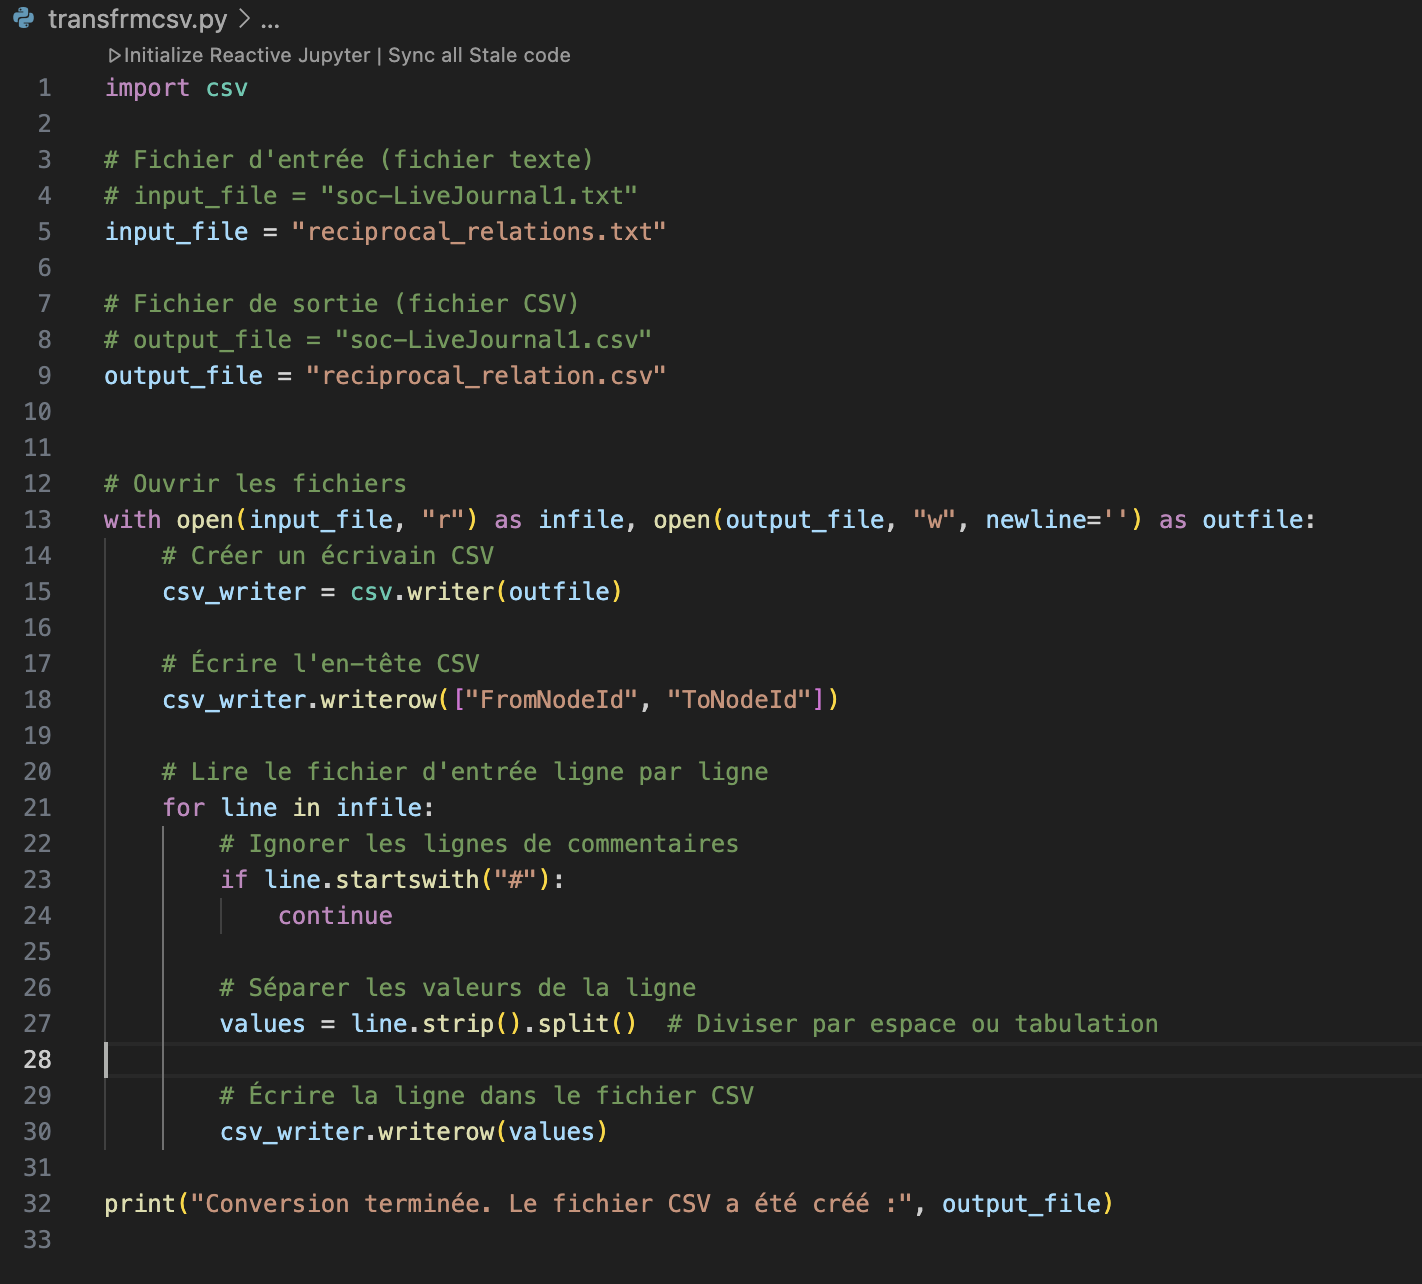
\includegraphics[width=0.5\textwidth]{transfrmcsv.png}
        \caption{Script transformation en CSV}
        \label{fig:label_image}
      \end{figure}

    \subsubsection{Suppression des boucles}
    Nous avons utilisé cette fonction proposée par networxX afin d'enlever les boucles du graphe. 

    \begin{figure}[h]
        \centering
        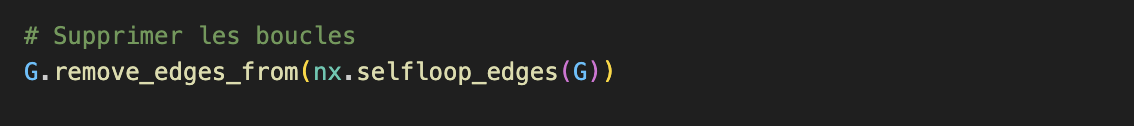
\includegraphics[width=0.5\textwidth]{Supp Boucles.png}
        \caption{Suppression des boucles}
        \label{fig:label_image}
    \end{figure}

    \subsubsection{Prise en compte uniquement des relation réciproque}
    Afin de garder une certaine cohérence dans nos données, nous avons fait le choix de garder uniquement les relations réciproques, c'est-à-dire les gens qui se suivent mutuellement. Pour ce faire, nous avons créé un script Python permettant de générer un fichier CSV contenant uniquement les nœuds réciproques (ce qui peut aussi pallier le biais des influenceurs, c'est-à-dire des gens qui sont suivis par beaucoup de monde mais qui ne suivent pas autant en retour).

        \begin{figure}[h]
            \centering
            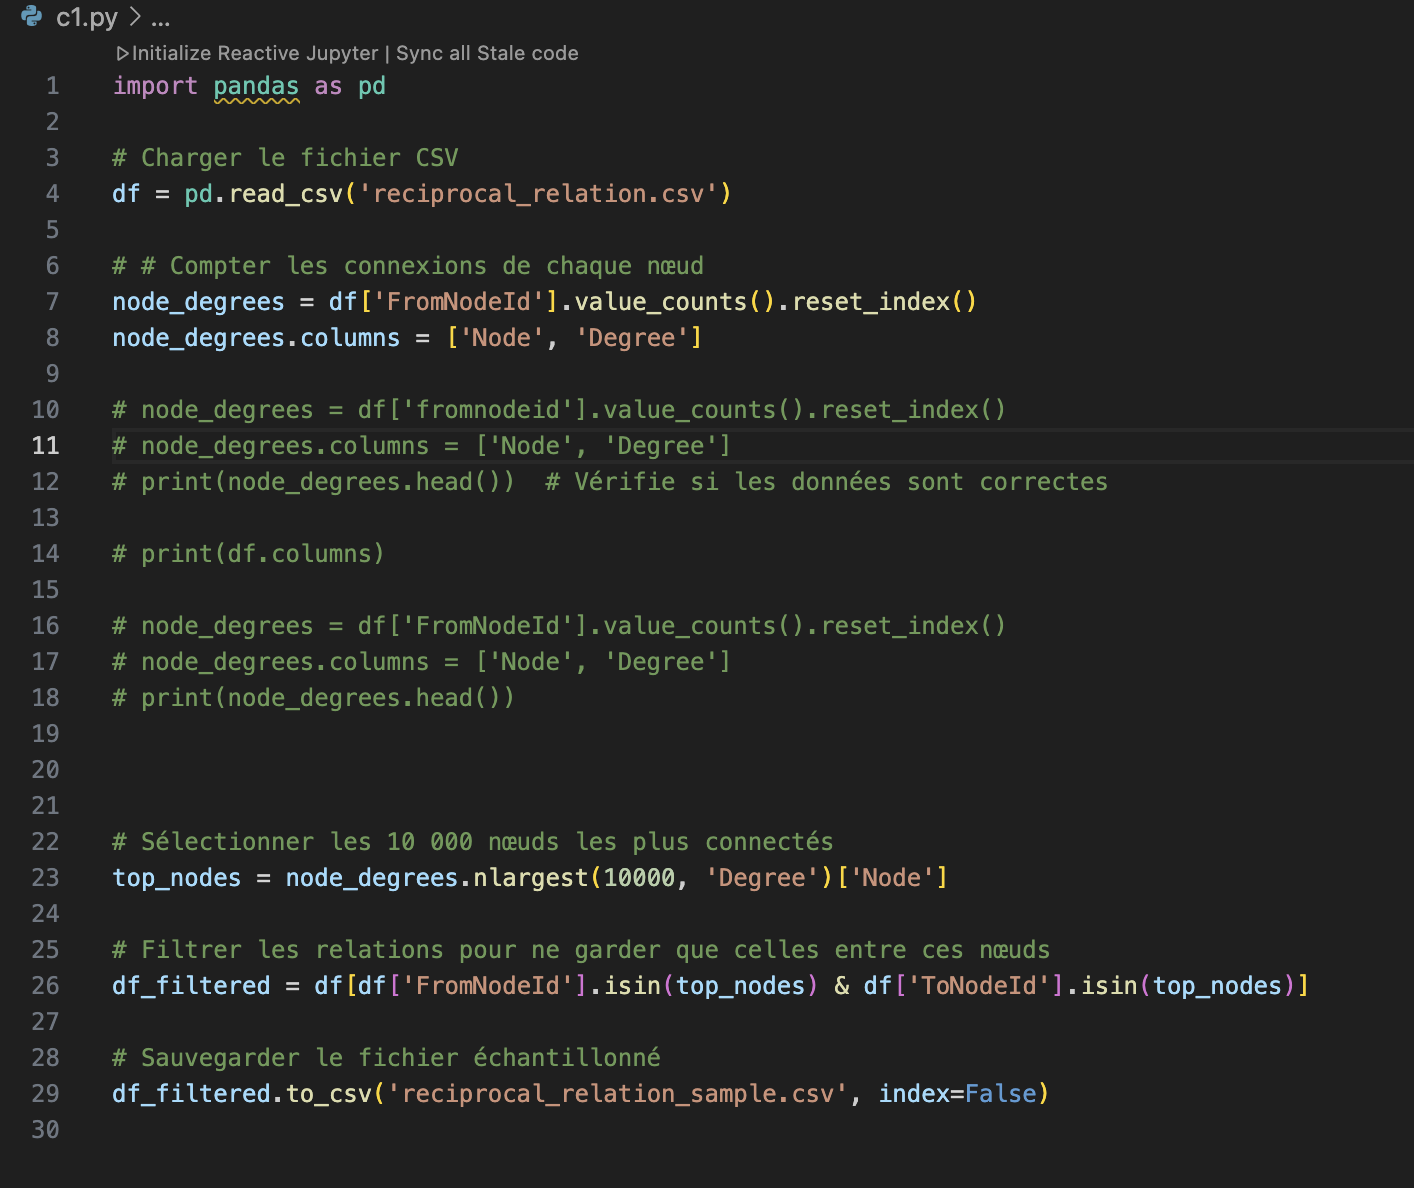
\includegraphics[width=0.5\textwidth]{reciproque.png}
            \caption{relation réciproque}
            \label{fig:label_image}
        \end{figure}

\newpage
    \subsection{Algorithme de parcours dans le graphe}
    Étant donnée les limites matérielles auxquelles nous sommes confronté, nous ne pouvons pas générer le graphe entier avec tous les nœuds. Afin de palier à ce problème nous avons implémenté des algorithmes nous permettant de prendre des échantillons représentatif de notre population (les utilisateurs de ce réseau sociale) pour nos test.

    \subsubsection{Random Walk Sampling}
    Principe : on démarre à un nœud au hasard, puis on choisit un voisin au hasard à chaque étape.
        \begin{figure}[H]
            \centering        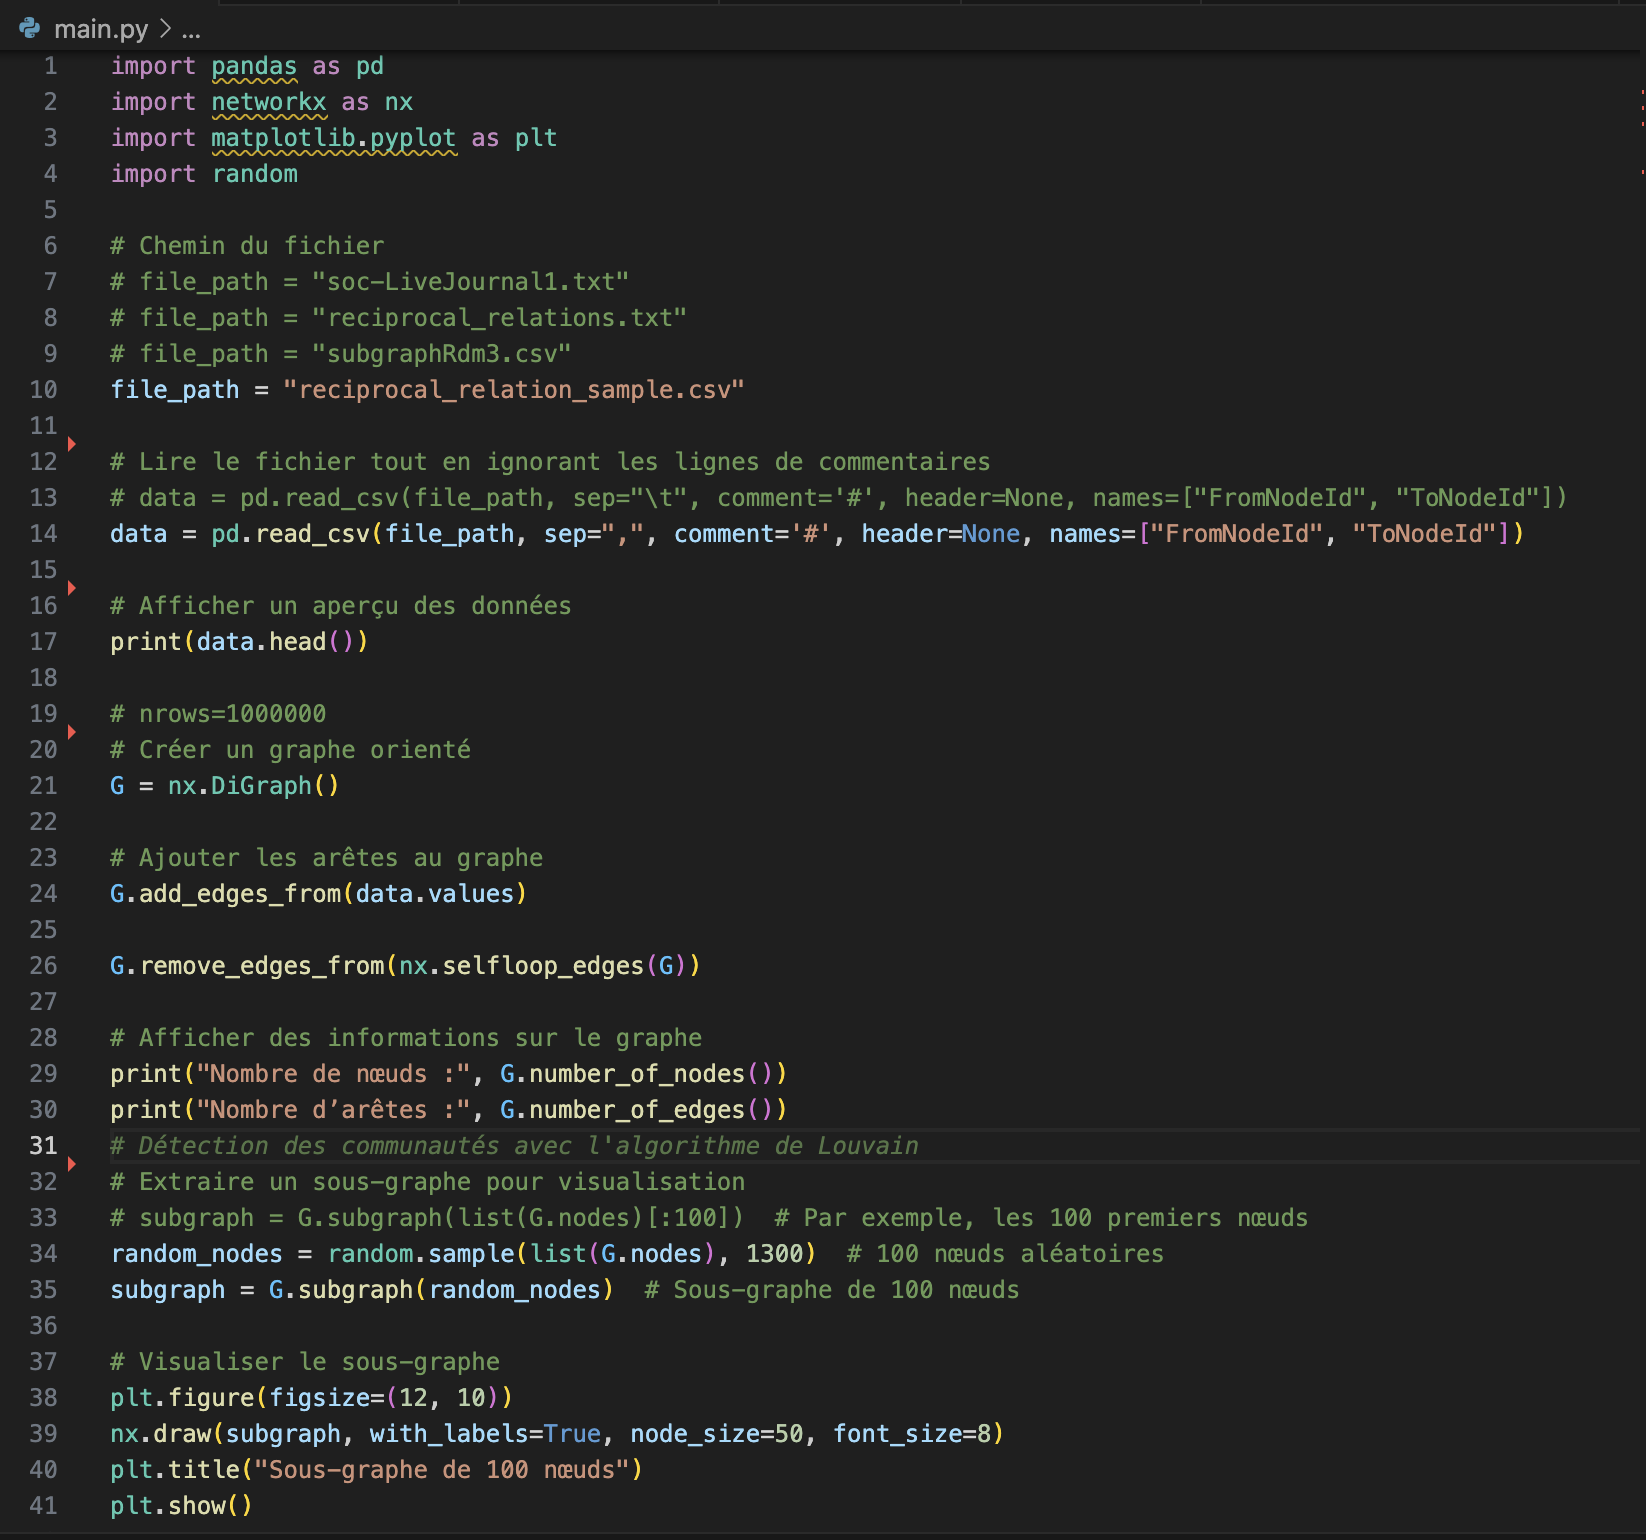
\includegraphics[width=0.5\textwidth]{Random Walk Sampling.png}
            \caption{Parcours aléatoire}
            \label{fig:label_image}
        \end{figure}

 
    \subsubsection{Induced Subgraph from High-Degree Nodes}
    On choisit quelques nœuds avec degré élevé + tous leurs voisins Intéressant pour cibler les "super connecteurs"

        \begin{figure}[H]
            \centering
            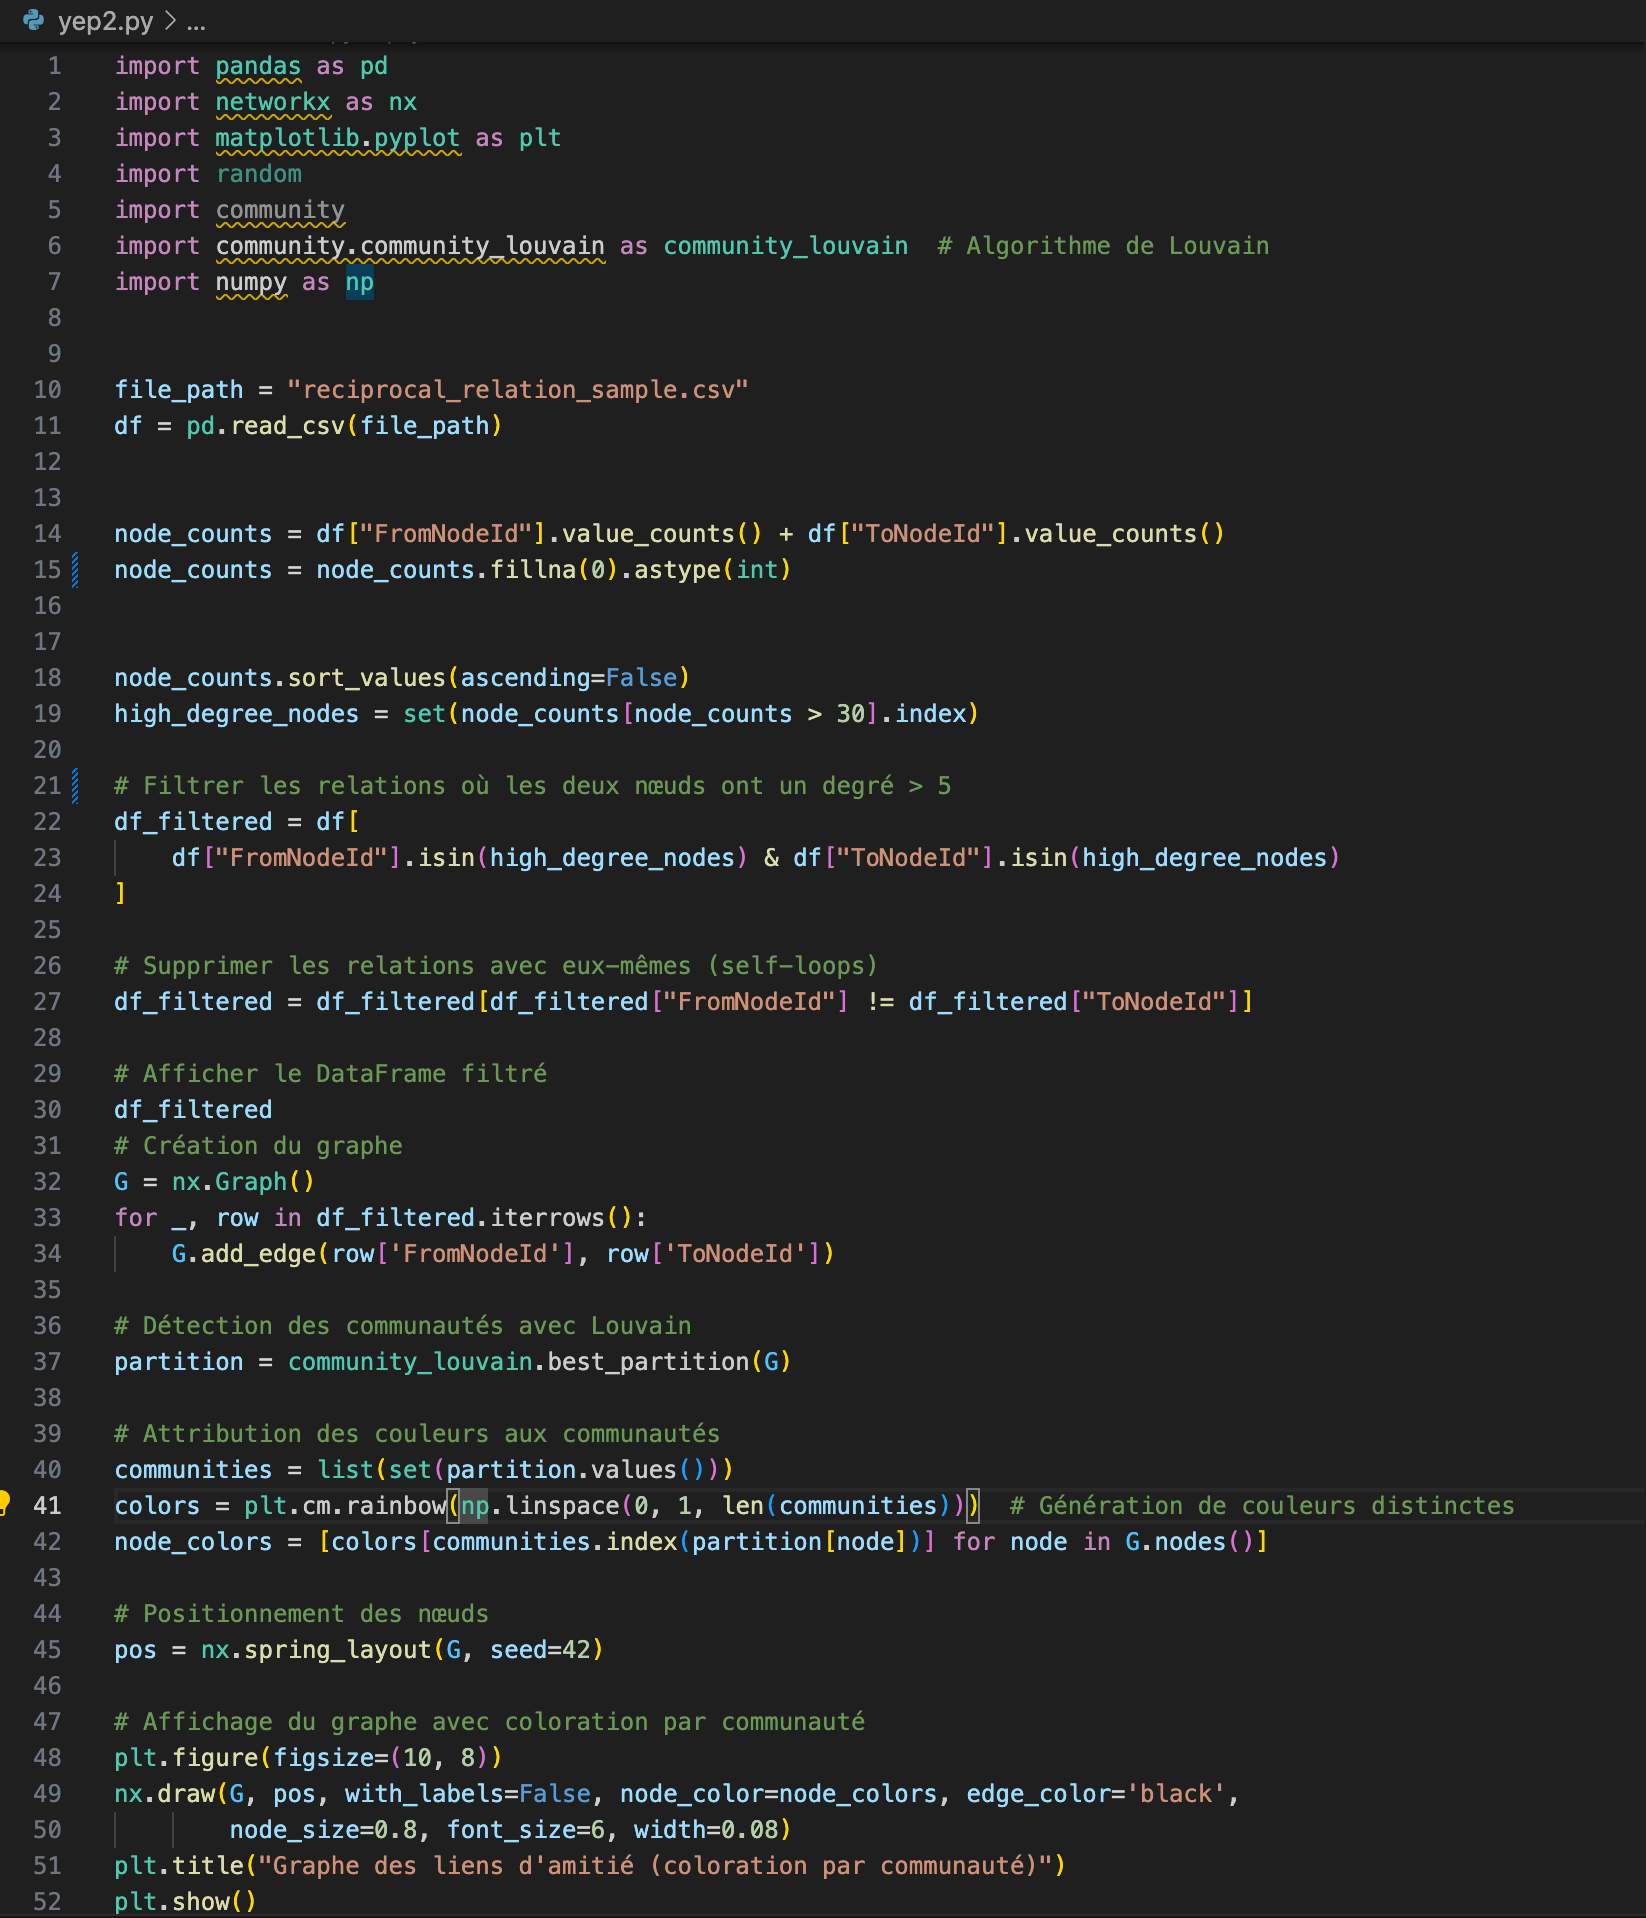
\includegraphics[width=0.5\textwidth]{degree.png}
            \caption{Script degré}
            \label{fig:label_image}
        \end{figure}

        \begin{figure}[H]
            \centering
            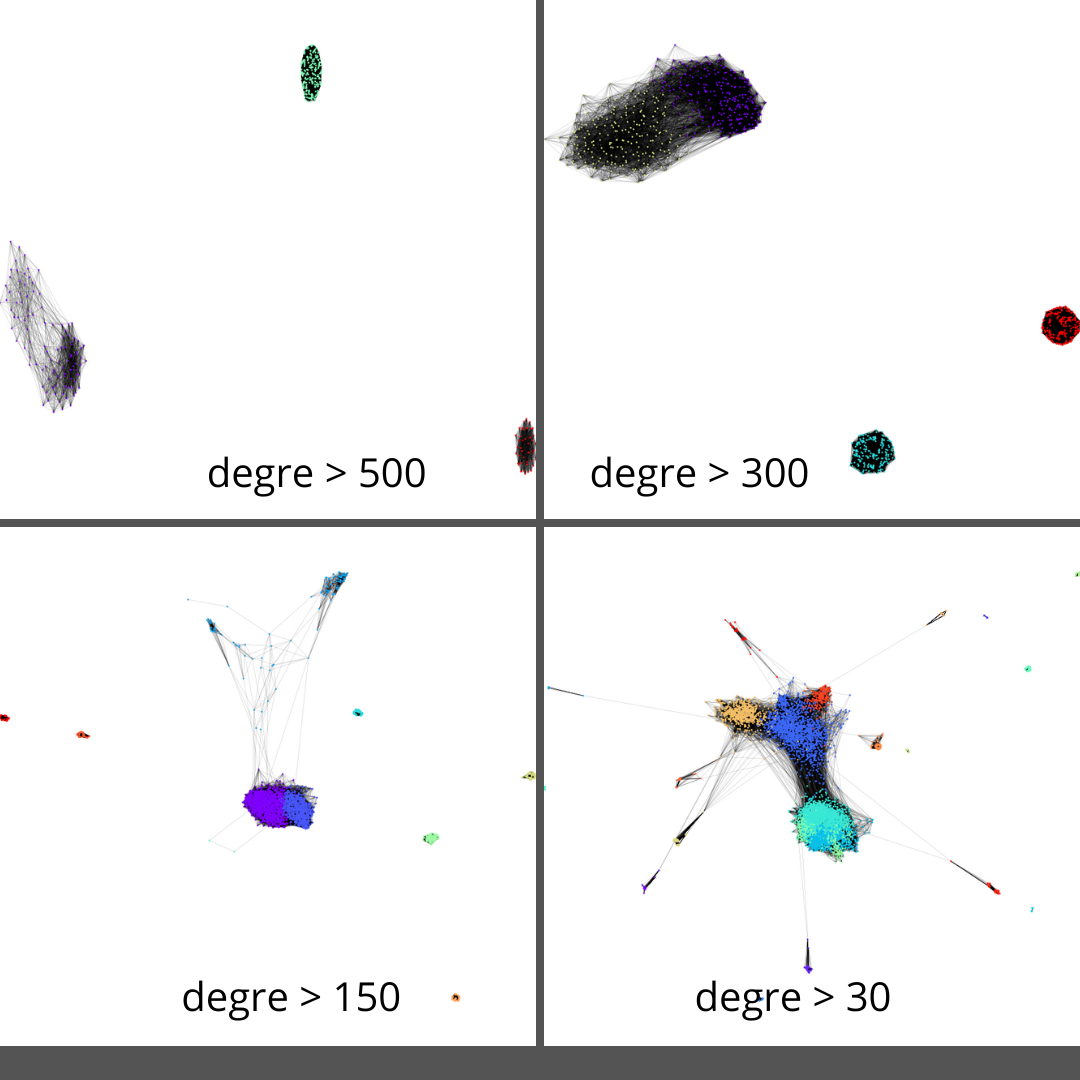
\includegraphics[width=0.5\textwidth]{degre graphe.png}
            \caption{degré graphe}
            \label{fig:label_image}
        \end{figure}
        
    \subsubsection{Breadth-First Search (BFS) Sampling}   
    Principe : on démarre à un nœud, on explore tous ses voisins, puis les voisins des voisins.
    Avantage : bon pour capturer une communauté locale
        \begin{figure}[H]
            \centering
            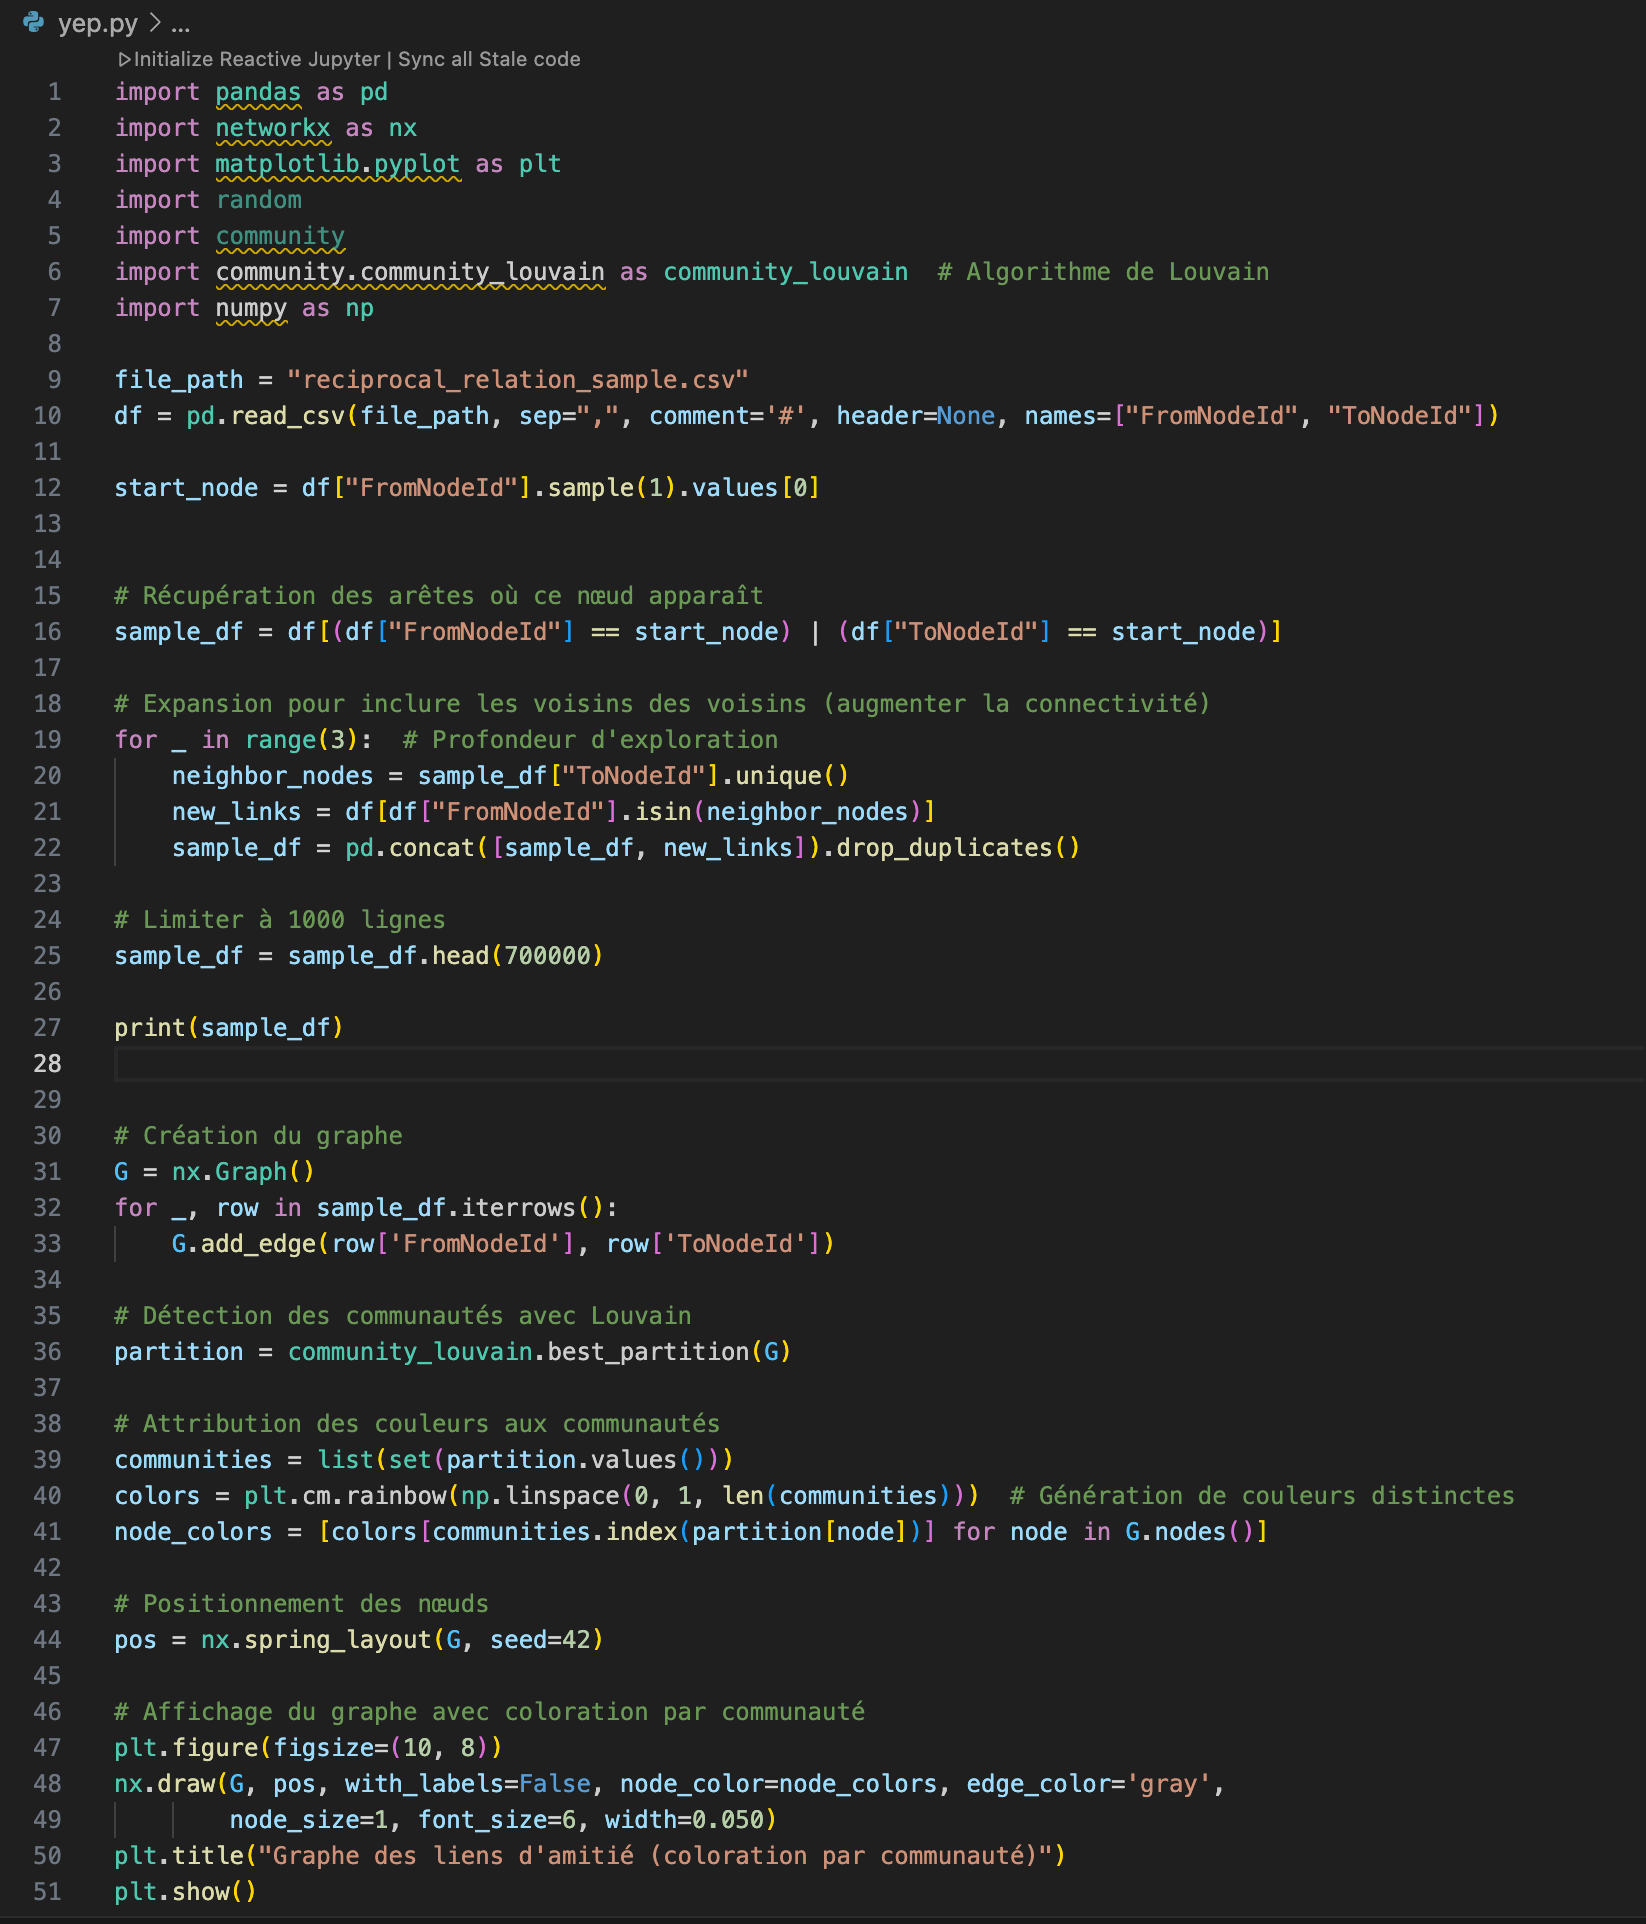
\includegraphics[width=0.5\textwidth]{voisin.png}
            \caption{Script Voisin}
            \label{fig:label_image}
        \end{figure}

        \begin{figure}[H]
            \centering
            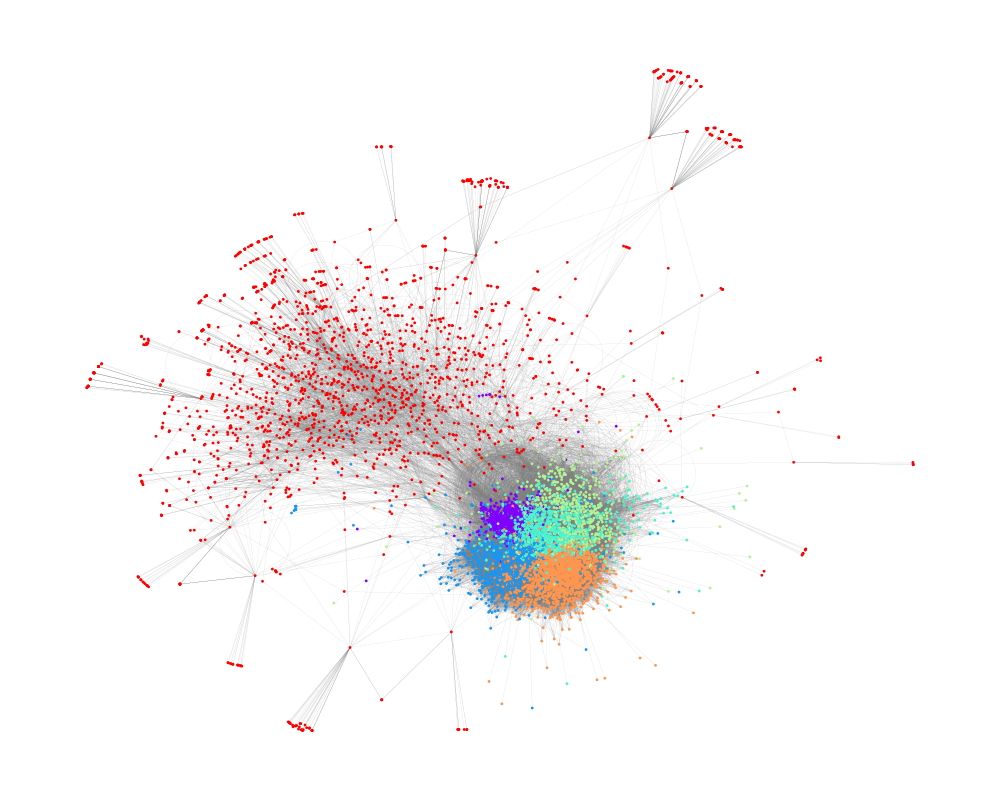
\includegraphics[width=0.5\textwidth]{voisin graphe.png}
            \caption{Voisin Graphe}
            \label{fig:label_image}
        \end{figure}


        \\
\newpage
    \subsection{Identification des communautés}
    - \textbf{Outils utilisés:}
    \begin{itemize}
        \item \texttt{Louvain Method} pour la détection des communautés, avec la librairie \texttt{community_louvain}.
        \item \texttt{NetworkX} pour la construction et l'analyse du graphe.
        \item \texttt{Matplotlib} et \texttt{Numpy} pour la visualisation et le traitement des couleurs des communautés.
    \end{itemize}
    
    - \textbf{Détails:}
    Les communautés dans le graphe sont identifiées à l'aide de la méthode de Louvain, qui optimise la modularité pour déterminer des groupes de nœuds fortement connectés entre eux. Cette approche permet de diviser le graphe en sous-graphes denses tout en maximisant la séparation entre ces groupes.

\subsection{Détermination des ponts reliant plusieurs communautés}
    - \textbf{Outils utilisés:}
    \begin{itemize}
        \item Détection des ponts via \texttt{NetworkX}, qui analyse les connexions entre les communautés pour identifier les nœuds qui relient des communautés distinctes.
        \item \texttt{Spring layout} de \texttt{NetworkX} pour positionner les nœuds de manière intuitive.
    \end{itemize}
    
    - \textbf{Détails:}
    Les nœuds ponts sont détectés comme étant des nœuds qui connectent des communautés différentes. Pour chaque nœud, nous vérifions s'il existe des voisins appartenant à une communauté différente. Ces nœuds jouent un rôle clé dans la transmission d'informations entre les communautés et sont donc essentiels pour comprendre les dynamiques globales du réseau.

\subsection{Identification des nœuds relais}
    - \textbf{Outils utilisés:}
    \begin{itemize}
        \item Sélection des nœuds relais parmi les nœuds ayant une forte centralité (degré élevé) et appartenant à des communautés différentes.
        \item \texttt{Random.shuffle()} pour sélectionner de manière aléatoire certains voisins intra-communauté pour l'esthétique de la visualisation.
    \end{itemize}
    
    - \textbf{Détails:}
    Les nœuds relais sont les nœuds qui servent de point de connexion entre différentes communautés. Nous avons sélectionné les \textit{top-k nœuds ponts} par communauté, où \(k\) est un paramètre défini, afin de limiter le nombre de nœuds à afficher tout en maintenant une représentation significative des connexions inter-communautés. Ces nœuds sont cruciaux pour faciliter les échanges d'informations à travers le réseau.

\subsection{Interprétation}
    - \textbf{Outils utilisés:}
    \begin{itemize}
        \item Visualisation du graphe via \texttt{Matplotlib} et \texttt{NetworkX}.
        \item Utilisation de la palette de couleurs \texttt{rainbow} pour distinguer les différentes communautés.
    \end{itemize}
    
    - \textbf{Détails:}
    La visualisation montre les nœuds des différentes communautés avec des couleurs distinctes, tandis que les nœuds ponts, qui relient différentes communautés, sont mis en évidence. Les nœuds relais, ayant un degré élevé et un rôle de connecteurs entre les groupes, sont essentiels pour comprendre la structure du réseau. En observant le graphe, nous pouvons identifier les principales interactions entre les communautés et les nœuds influents qui jouent un rôle crucial dans la circulation de l'information au sein du réseau.


\section{Bibliothèques, Outils et technologies}
\section{Travail réalisé}

\subsection{Script Python permettant de nettoyer nos données}

Pour filtrer les données en raison de leur grande taille, nous avons choisi de ne conserver que les relations réciproques, c’est-à-dire celles où deux individus s'influencent mutuellement. Par exemple, si A suit B et que B suit également A, cette relation est maintenue. En revanche, si A suit C mais que C ne suit pas A, cette relation est supprimée, car elle n’est pas réciproque. De plus, nous avons éliminé toutes les relations où un individu suit lui-même, c'est-à-dire les relations de type "A suit A". Ce filtrage permet de réduire la taille des données et de conserver uniquement les interactions mutuelles pertinentes.

\subsection{algorithmes de parcours}
- Random Walk Sampling\\
- Induced Subgraph from High-Degree Nodes\\
- Breadth-First Search (BFS) Sampling\\

\newpage
\section{Détection de communautés}

Le script Python présenté ci-dessous permet de détecter des communautés dans un réseau social à partir de relations réciproques. Il filtre d'abord les données en ne gardant que les nœuds ayant un degré supérieur à 30 et les relations réciproques entre ces nœuds, en éliminant les relations où un nœud suit lui-même. Ensuite, un graphe est construit avec ces données filtrées. L'algorithme de Louvain est utilisé pour détecter les communautés.

\begin{lstlisting}
import pandas as pd
import networkx as nx
import matplotlib.pyplot as plt
import community  
import community.community_louvain as community_louvain
import numpy as np 

file_path = "reciprocal_relation_sample.csv"
df = pd.read_csv(file_path)

node_counts = df["FromNodeId"].value_counts() + df["ToNodeId"].value_counts()
node_counts = node_counts.fillna(0).astype(int)

node_counts.sort_values(ascending=False)
high_degree_nodes = set(node_counts[node_counts > 30].index)

df_filtered = df[
    df["FromNodeId"].isin(high_degree_nodes) & df["ToNodeId"].isin(high_degree_nodes)
]

df_filtered = df_filtered[df_filtered["FromNodeId"] != df_filtered["ToNodeId"]]

G = nx.Graph()
for _, row in df_filtered.iterrows():
    G.add_edge(row['FromNodeId'], row['ToNodeId'])

partition = community_louvain.best_partition(G)

communities = list(set(partition.values()))
colors = plt.cm.rainbow(np.linspace(0, 1, len(communities)))
node_colors = [colors[communities.index(partition[node])] for node in G.nodes()]

pos = nx.spring_layout(G, seed=42)

plt.figure(figsize=(10, 8))
nx.draw(G, pos, with_labels=False, node_color=node_colors, edge_color='black',
        node_size=0.8, font_size=6, width=0.08)
plt.title("Graphe des liens d'amitié (coloration par communauté)")
plt.show()
\end{lstlisting}

\newpage
\subsection{Résultats aperçus}

Après l'application de l'algorithme de Louvain, nous obtenons un graphe où chaque nœud représente un individu et les arêtes entre les nœuds représentent les relations réciproques. Les nœuds sont colorés en fonction des communautés auxquelles ils appartiennent, facilitant la visualisation des groupes interagissant fortement.

\begin{figure}[H]
    \centering
    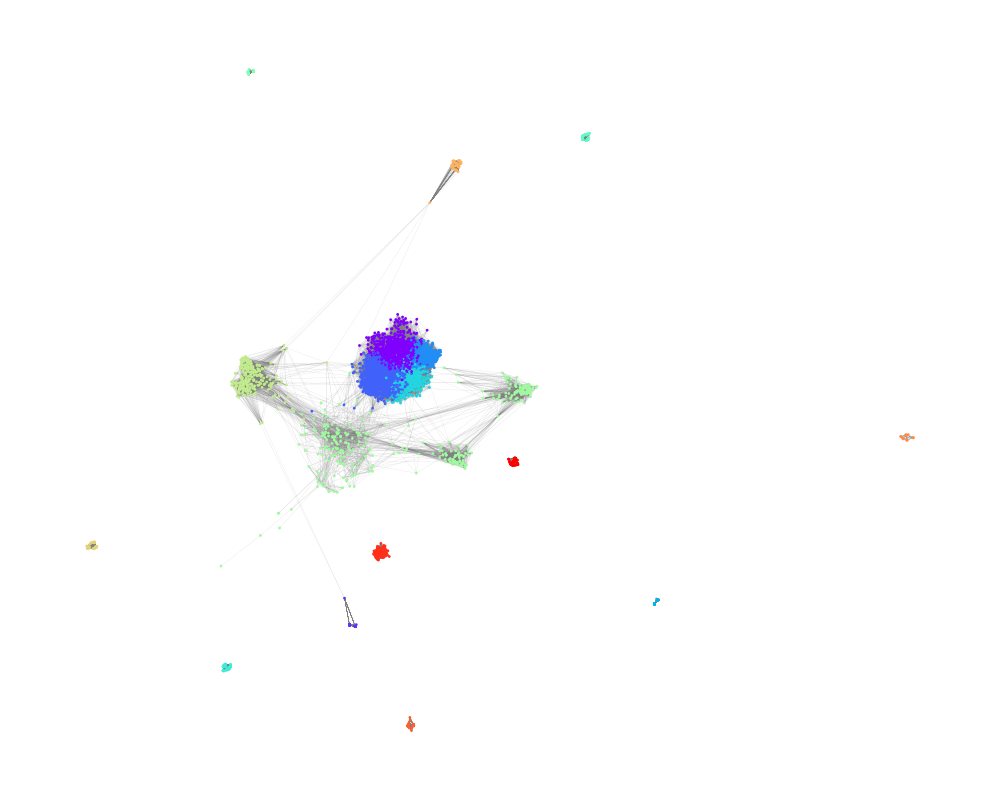
\includegraphics[width=0.85\textwidth]{detection_communaute.png}
    \caption{Détection des communautés dans le réseau d'amitié}
    \label{fig:communaute}
\end{figure}

\newpage
\subsection{Analyse des liens inter-communautés et des nœuds ponts}

Dans cette section, nous analysons les liens inter-communautés et identifions les nœuds ponts. Ces derniers sont essentiels pour relier différentes communautés et favoriser la circulation de l'information. Voici le code Python permettant de détecter et visualiser ces nœuds.

\begin{lstlisting}
# Identification des nœuds ponts
bridge_nodes = set()
for node in G.nodes():
    comm = partition[node]
    for neighbor in G.neighbors(node):
        if partition[neighbor] != comm:
            bridge_nodes.add(node)
            break

# Visualisation des connexions inter-communautés
pos = nx.spring_layout(G, seed=42)
subG = G.subgraph(bridge_nodes)
node_colors = [colors[communities.index(partition[node])] for node in subG.nodes()]

plt.figure(figsize=(12, 10))
nx.draw_networkx_nodes(subG, pos, node_color=node_colors, node_size=50)
nx.draw_networkx_edges(subG, pos, edge_color='black', width=0.4)
plt.title("Connexions entre communautés via les nœuds ponts")
plt.axis("off")
plt.tight_layout()
plt.savefig("inter_community_links.png", dpi=300)
plt.show()
\end{lstlisting}

\begin{figure}[H]
    \centering
    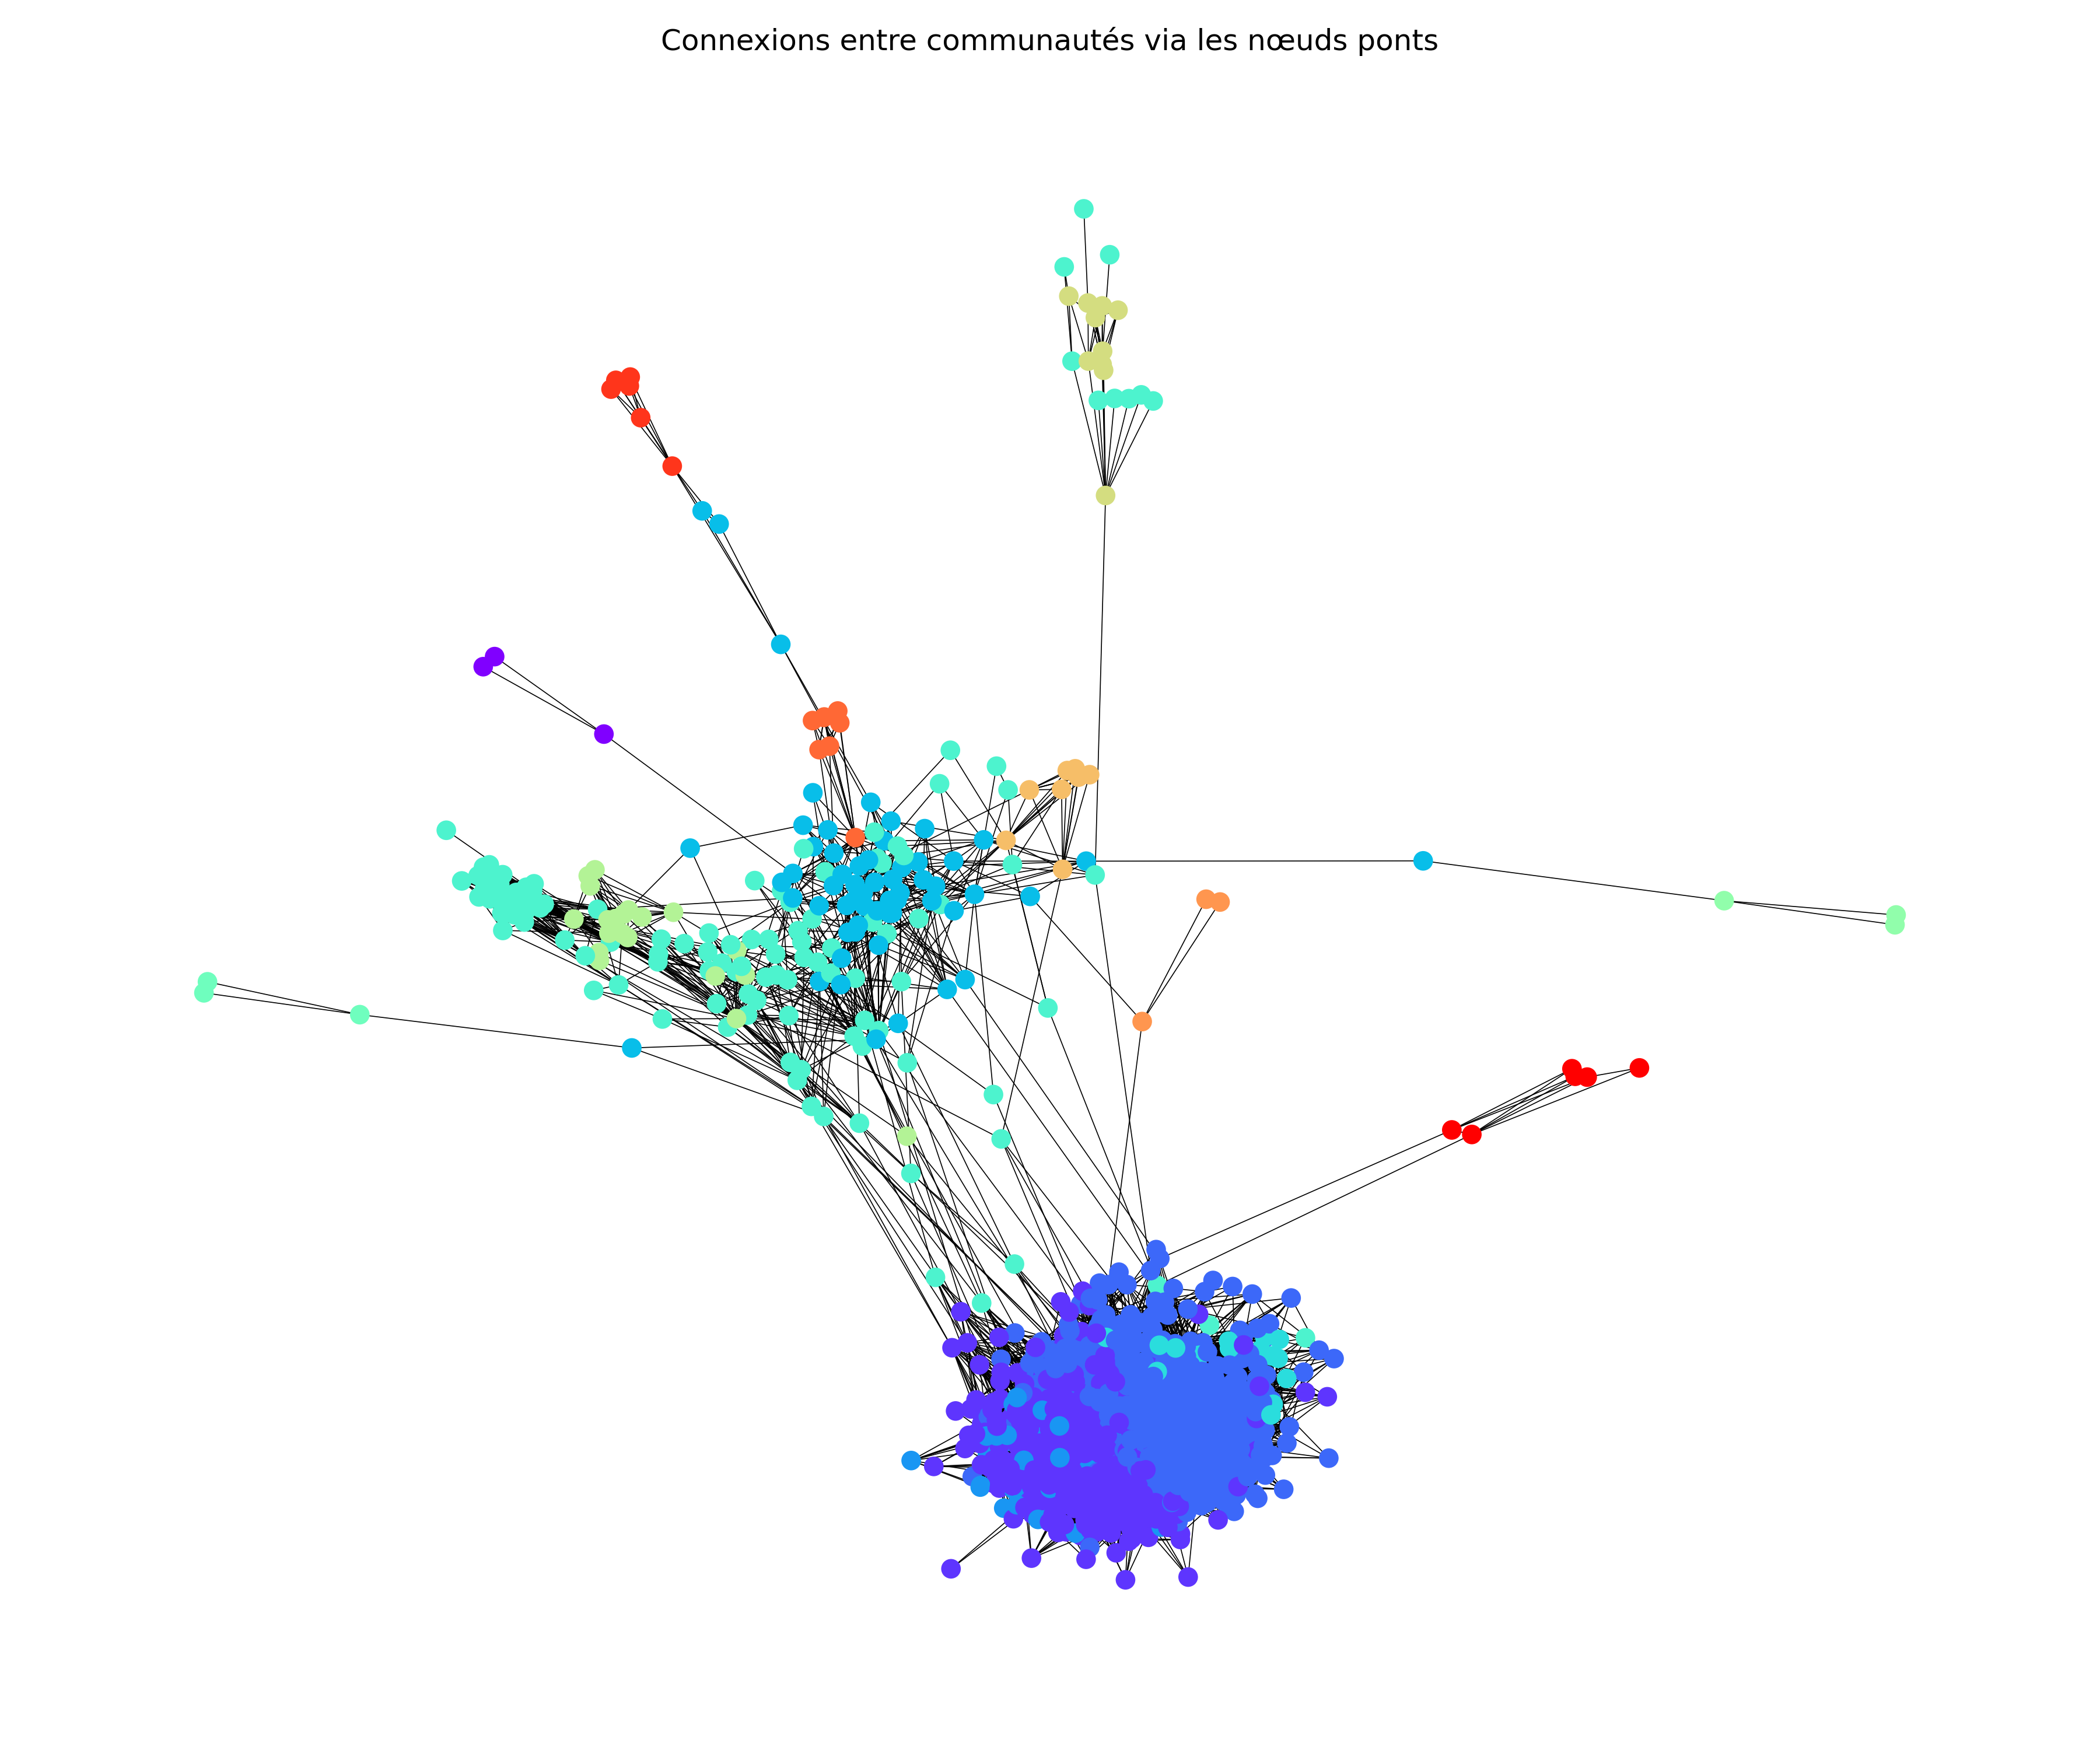
\includegraphics[width=0.85\textwidth]{inter_community_links.png}
    \caption{Liens inter-communautés via les nœuds ponts}
    \label{fig:inter_community_links}
\end{figure}

\newpage
\subsection{Identification et visualisation des connexions clés entre les communautés}

Pour mieux comprendre la dynamique globale du réseau, nous analysons dans cette section les \textbf{connexions inter-communautés}, c’est-à-dire les liens reliant des nœuds appartenant à des groupes différents. Ces connexions sont essentielles, car elles révèlent les points de contact stratégiques entre les communautés, souvent représentés par des nœuds occupant un rôle de liaison ou d'ambassadeur.

\vspace{1em}
Les étapes principales de cette analyse sont les suivantes :
\begin{itemize}
    \item Identifier les arêtes connectant des nœuds de communautés différentes.
    \item Extraire les sous-graphes formés par ces connexions inter-groupes.
    \item Générer une visualisation pour chaque paire de communautés connectées, en mettant en valeur les arêtes clés.
\end{itemize}

\vspace{1em}
Le script Python suivant a été utilisé pour mettre en œuvre cette analyse :

\begin{lstlisting}[language=Python, caption={Identification des connexions inter-communautés}, label={lst:intercomm}, frame=single, basicstyle=\ttfamily\small]
# Couleurs des communautés
unique_communities = sorted(set(partition.values()))
colors = plt.cm.rainbow(np.linspace(0, 1, len(unique_communities)))
community_color_map = {comm: colors[i] for i, comm in enumerate(unique_communities)}

# Détection des arêtes entre communautés
inter_edges = [
    (u, v, partition[u], partition[v]) for u, v in G.edges() if partition[u] != partition[v]
]

# Paires de communautés uniques
pairs = set((min(c1, c2), max(c1, c2)) for _, _, c1, c2 in inter_edges)

for comm1, comm2 in pairs:
    connector_nodes = set()
    edges_between = []

    for u, v, c1, c2 in inter_edges:
        if set([c1, c2]) == set([comm1, comm2]):
            connector_nodes.update([u, v])
            edges_between.append((u, v))

    # Ajout des voisins immédiats
    neighbor_nodes = set()
    for node in connector_nodes:
        neighbor_nodes.update(G.neighbors(node))

    total_nodes = connector_nodes.union(neighbor_nodes)
    subG = G.subgraph(total_nodes)

    # Position et couleurs
    pos = nx.spring_layout(subG, seed=42)
    node_colors = [community_color_map[partition[n]] for n in subG.nodes()]
    edge_colors = ['black' if (u, v) in edges_between or (v, u) in edges_between else 'gray'
                   for u, v in subG.edges()]

    # Dessin
    plt.figure(figsize=(10, 8))
    nx.draw_networkx_nodes(subG, pos, node_color=node_colors, node_size=100)
    nx.draw_networkx_edges(subG, pos, edge_color=edge_colors, width=1.5)
    plt.title(f"Connexions entre communautés {comm1} et {comm2}")
    plt.axis("off")
    plt.tight_layout()
    plt.savefig(f"liaison_{comm1}_{comm2}.png", dpi=300)
    plt.show()
\end{lstlisting}

\vspace{1em}
Les visualisations ci-dessous illustrent quelques-unes de ces connexions inter-communautaires identifiées :

\begin{figure}[H]
    \centering
    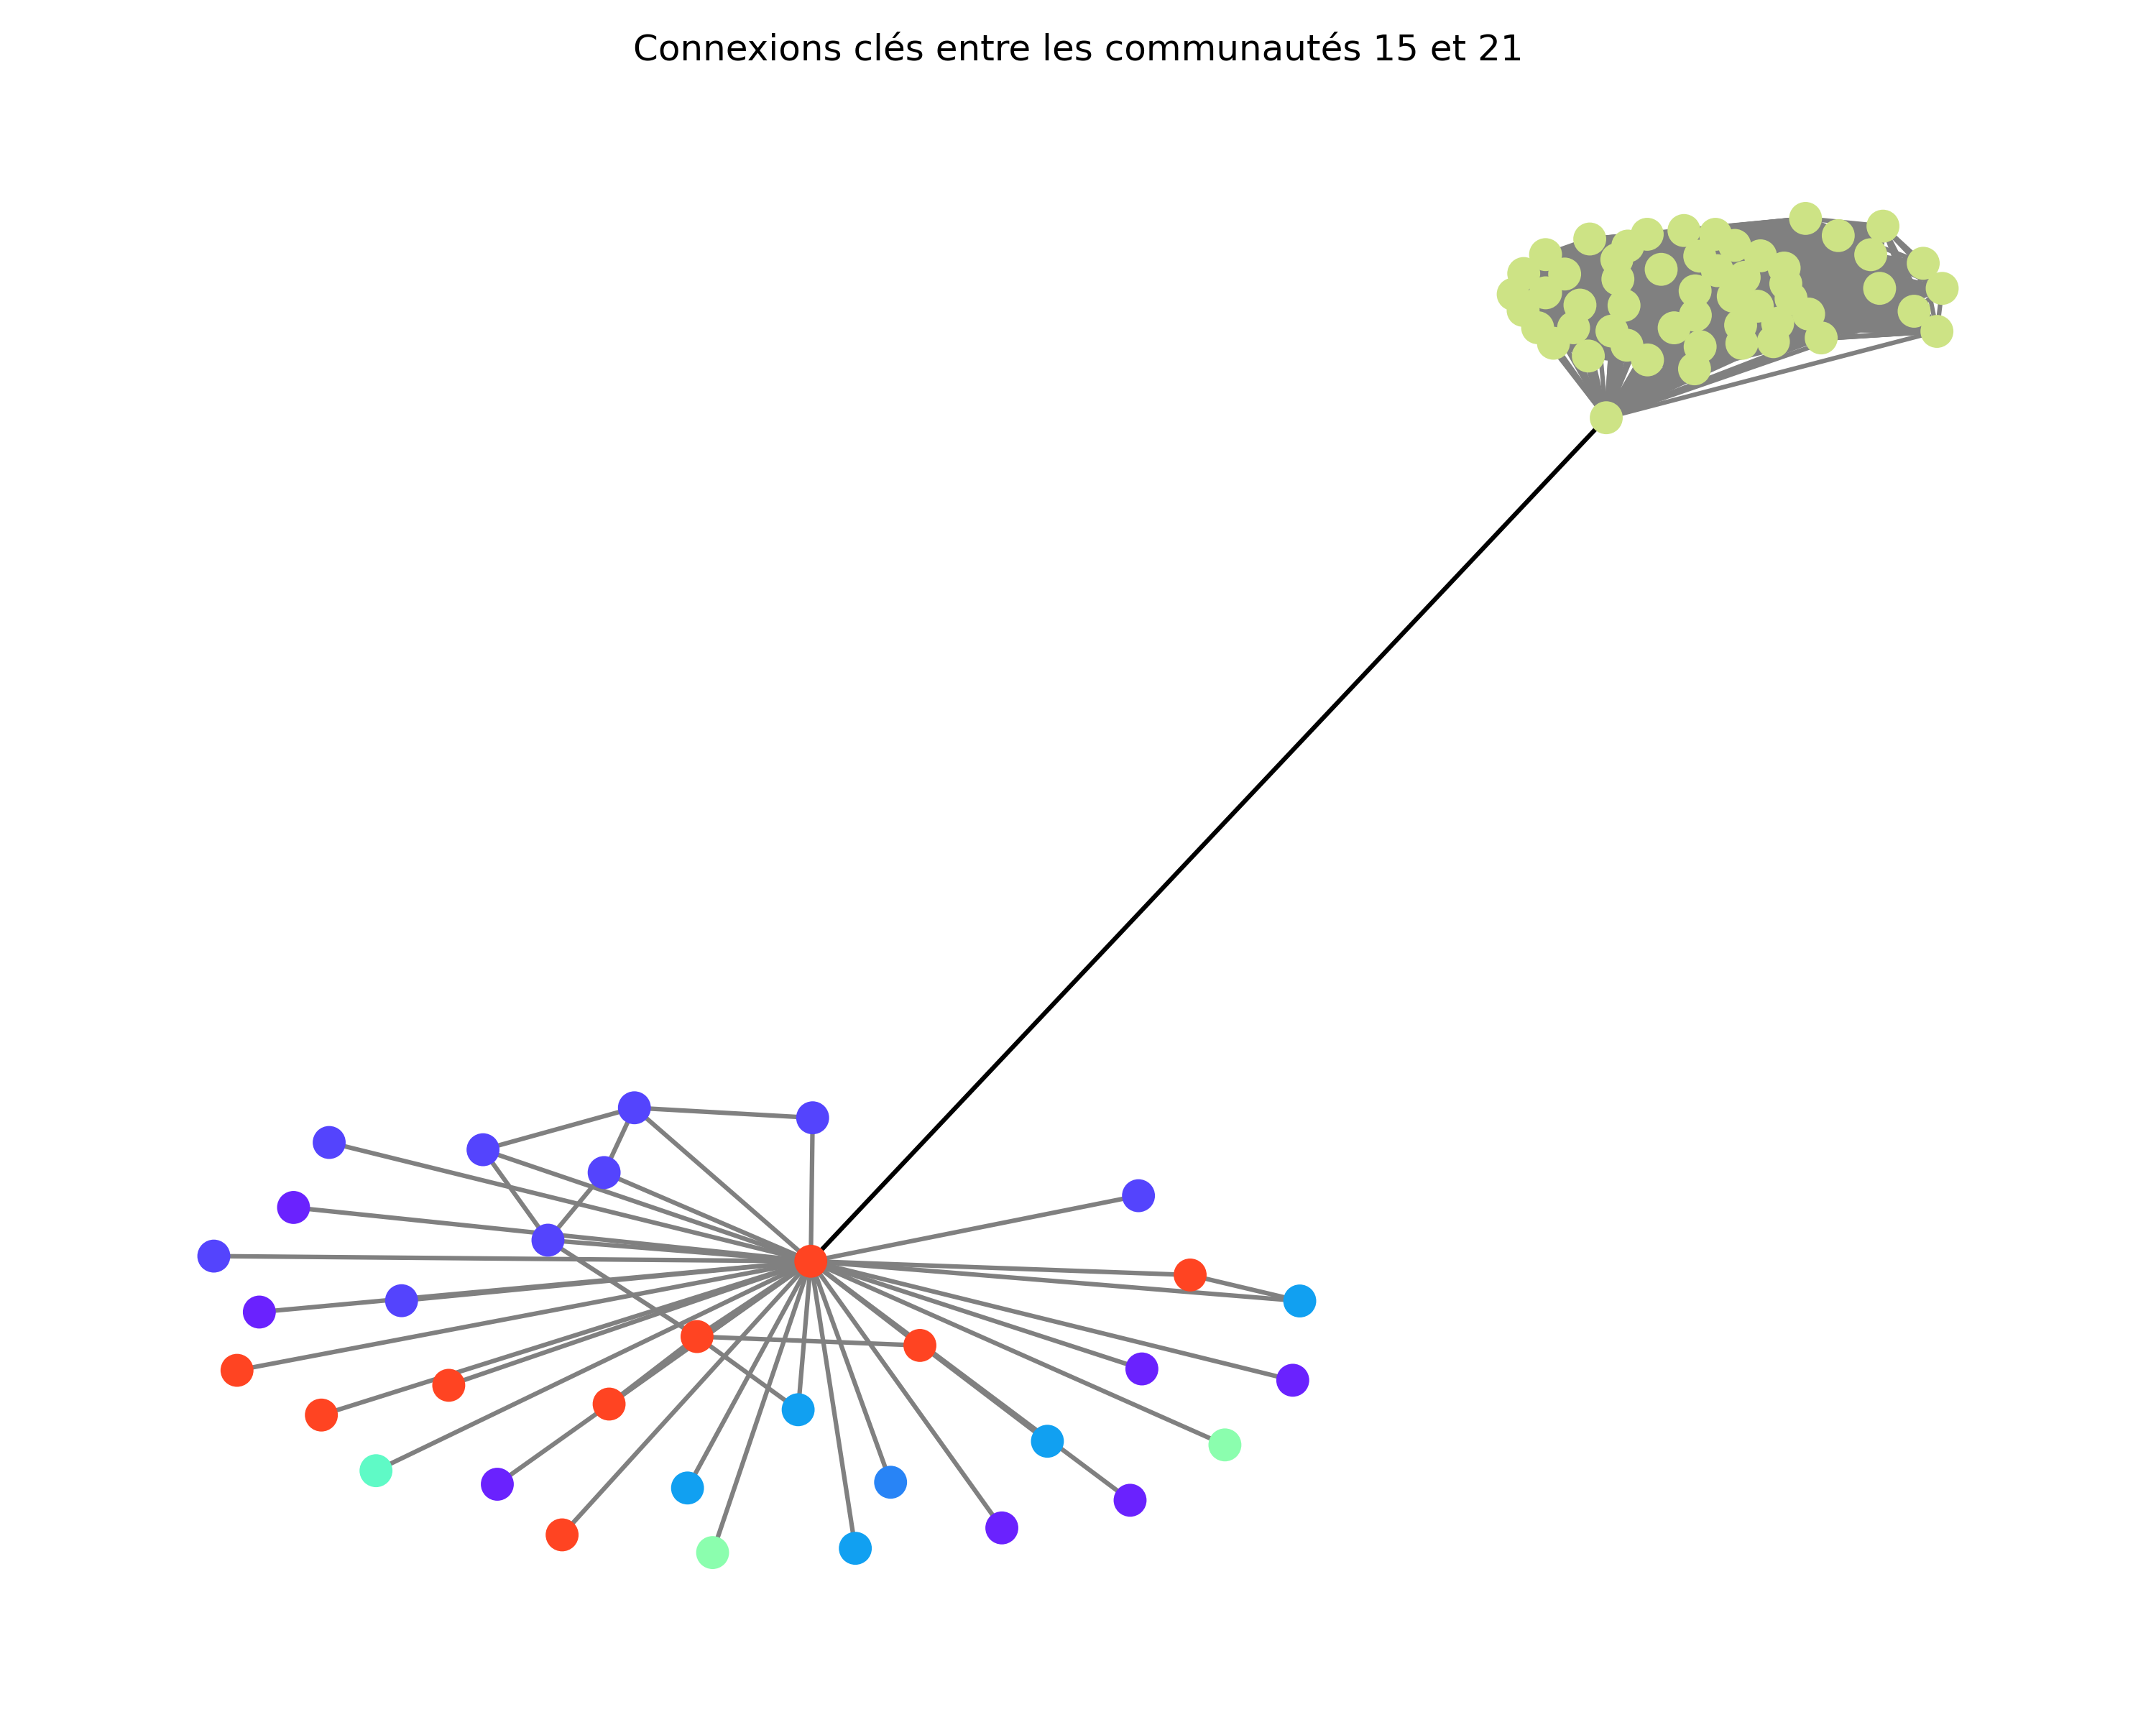
\includegraphics[width=0.8\textwidth]{liaison_15_21.png}
    \caption{Connexions clés entre les communautés 15 et 21}
    \label{fig:liaison_15_21}
\end{figure}

\begin{figure}[H]
    \centering
    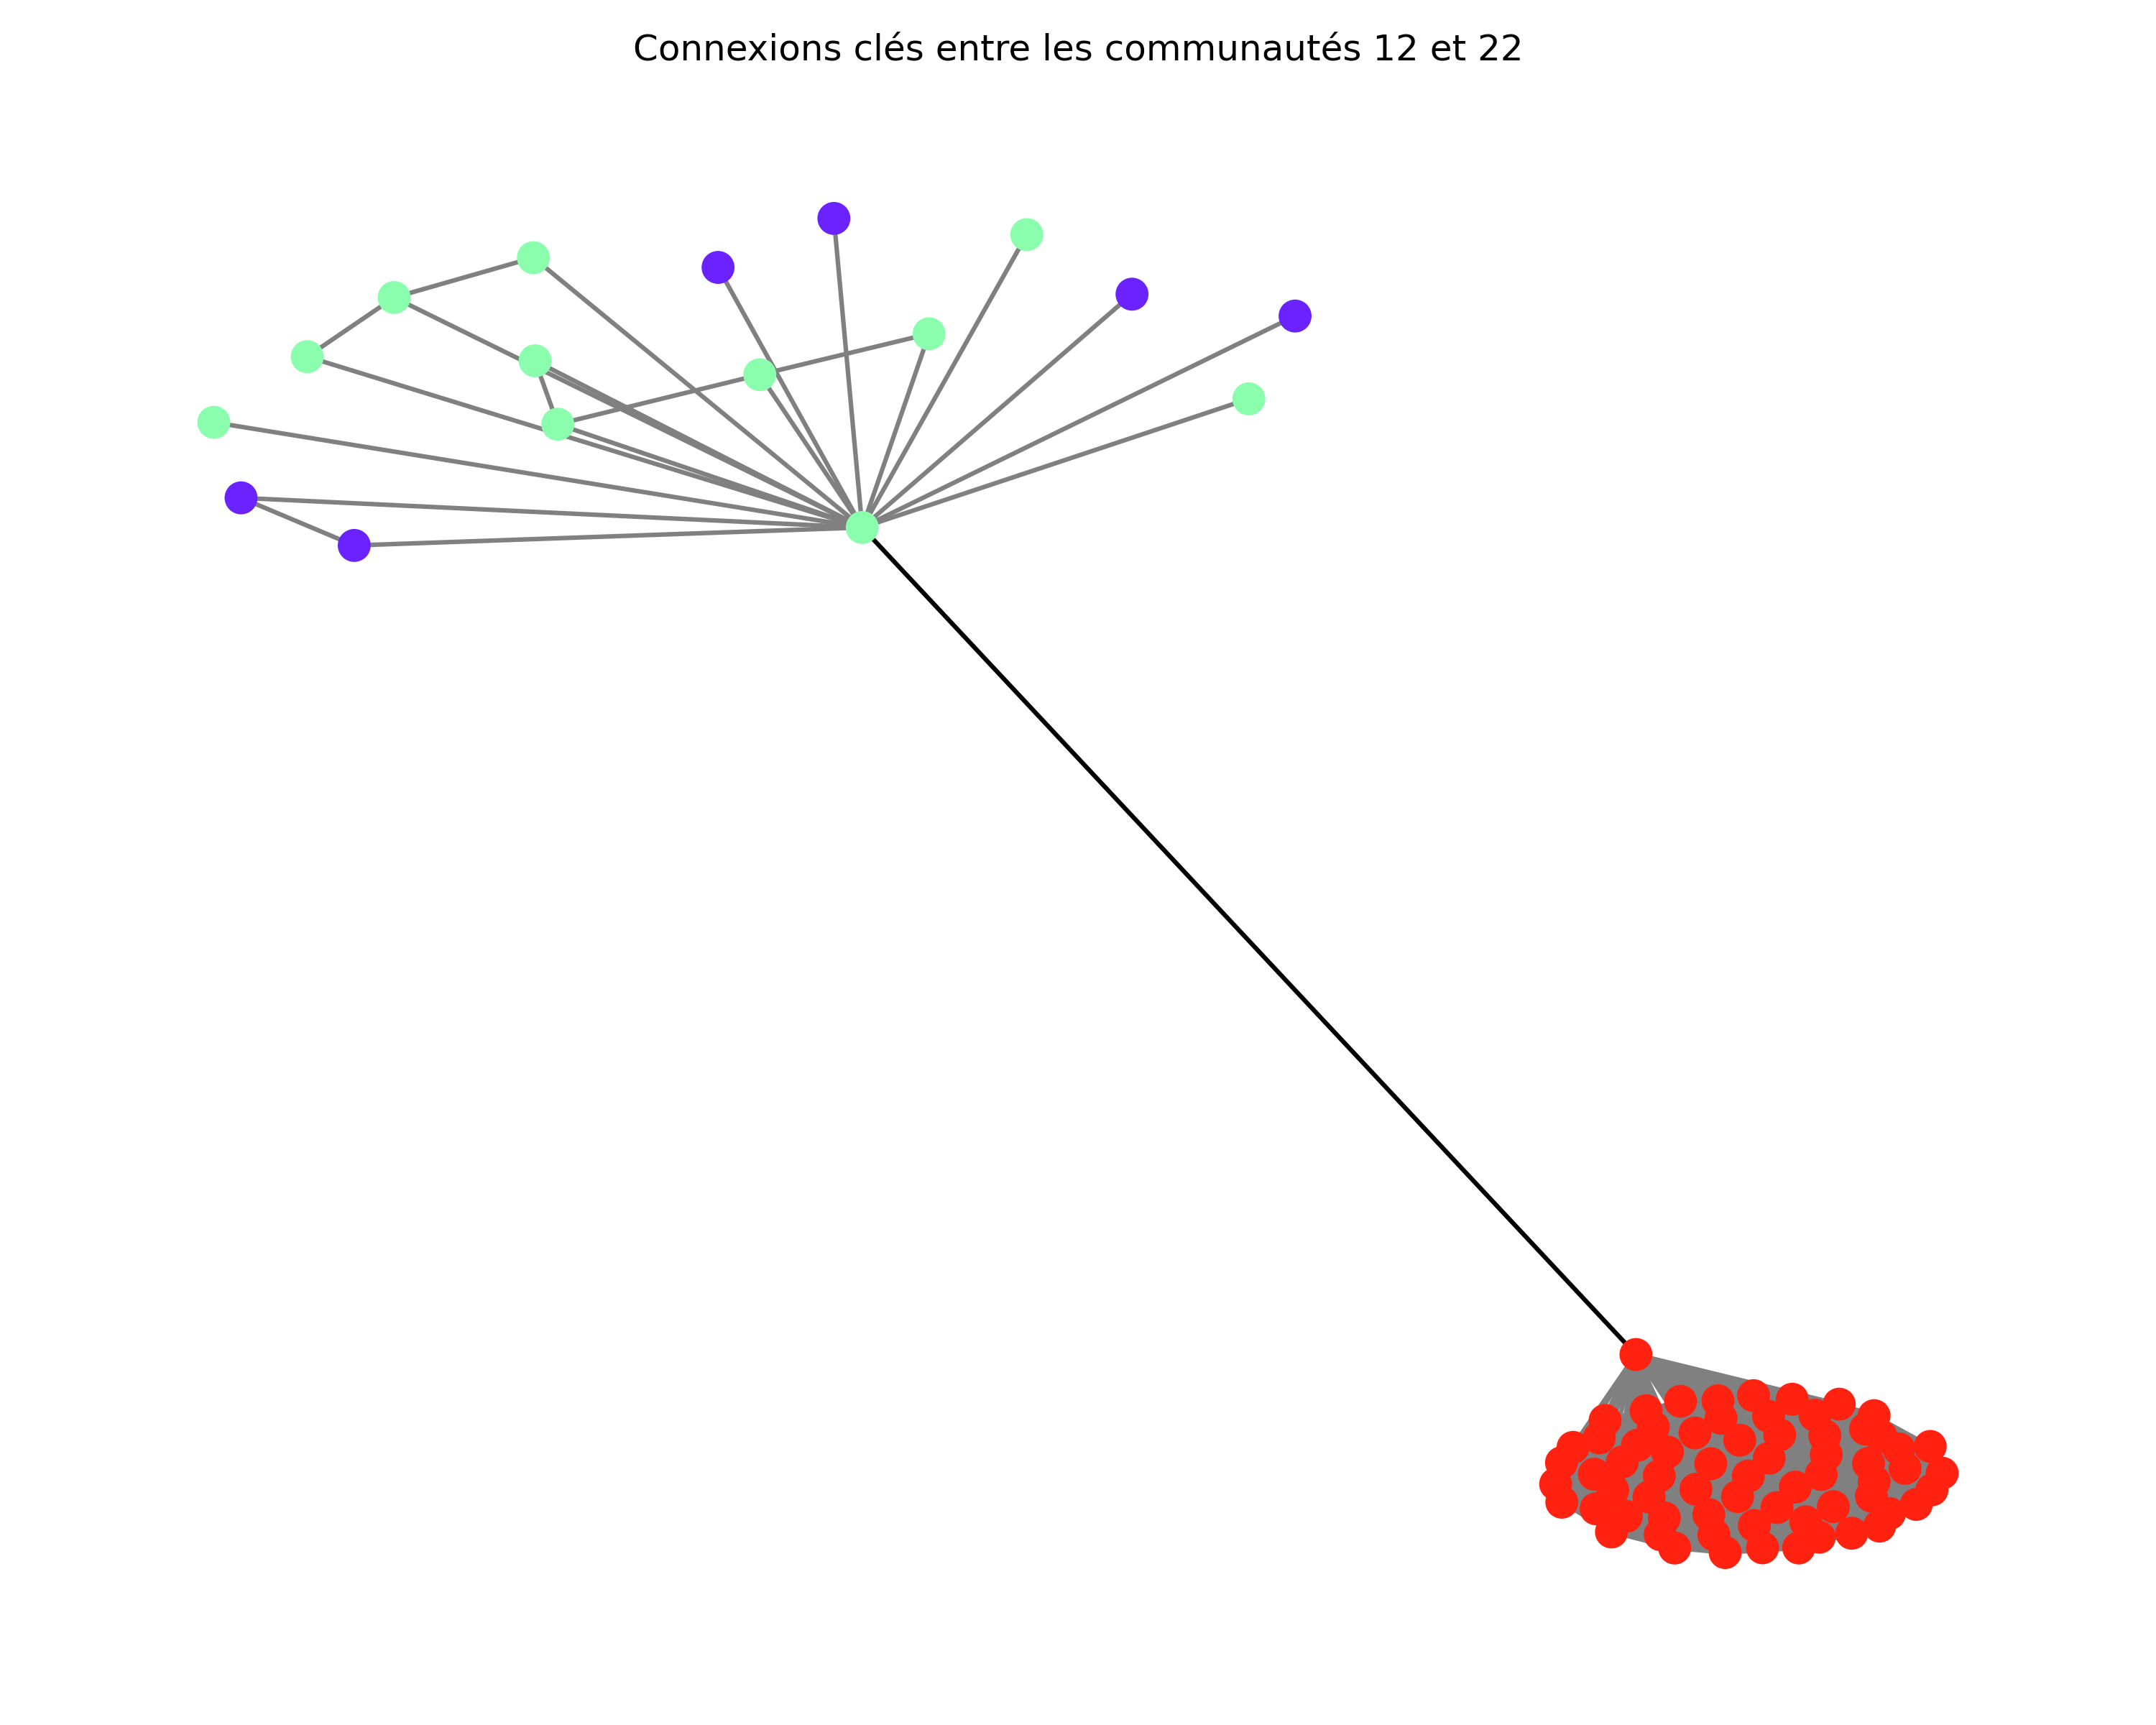
\includegraphics[width=0.8\textwidth]{liaison_12_22.png}
    \caption{Connexions clés entre les communautés 12 et 22}
    \label{fig:liaison_12_22}
\end{figure}

\begin{figure}[H]
    \centering
    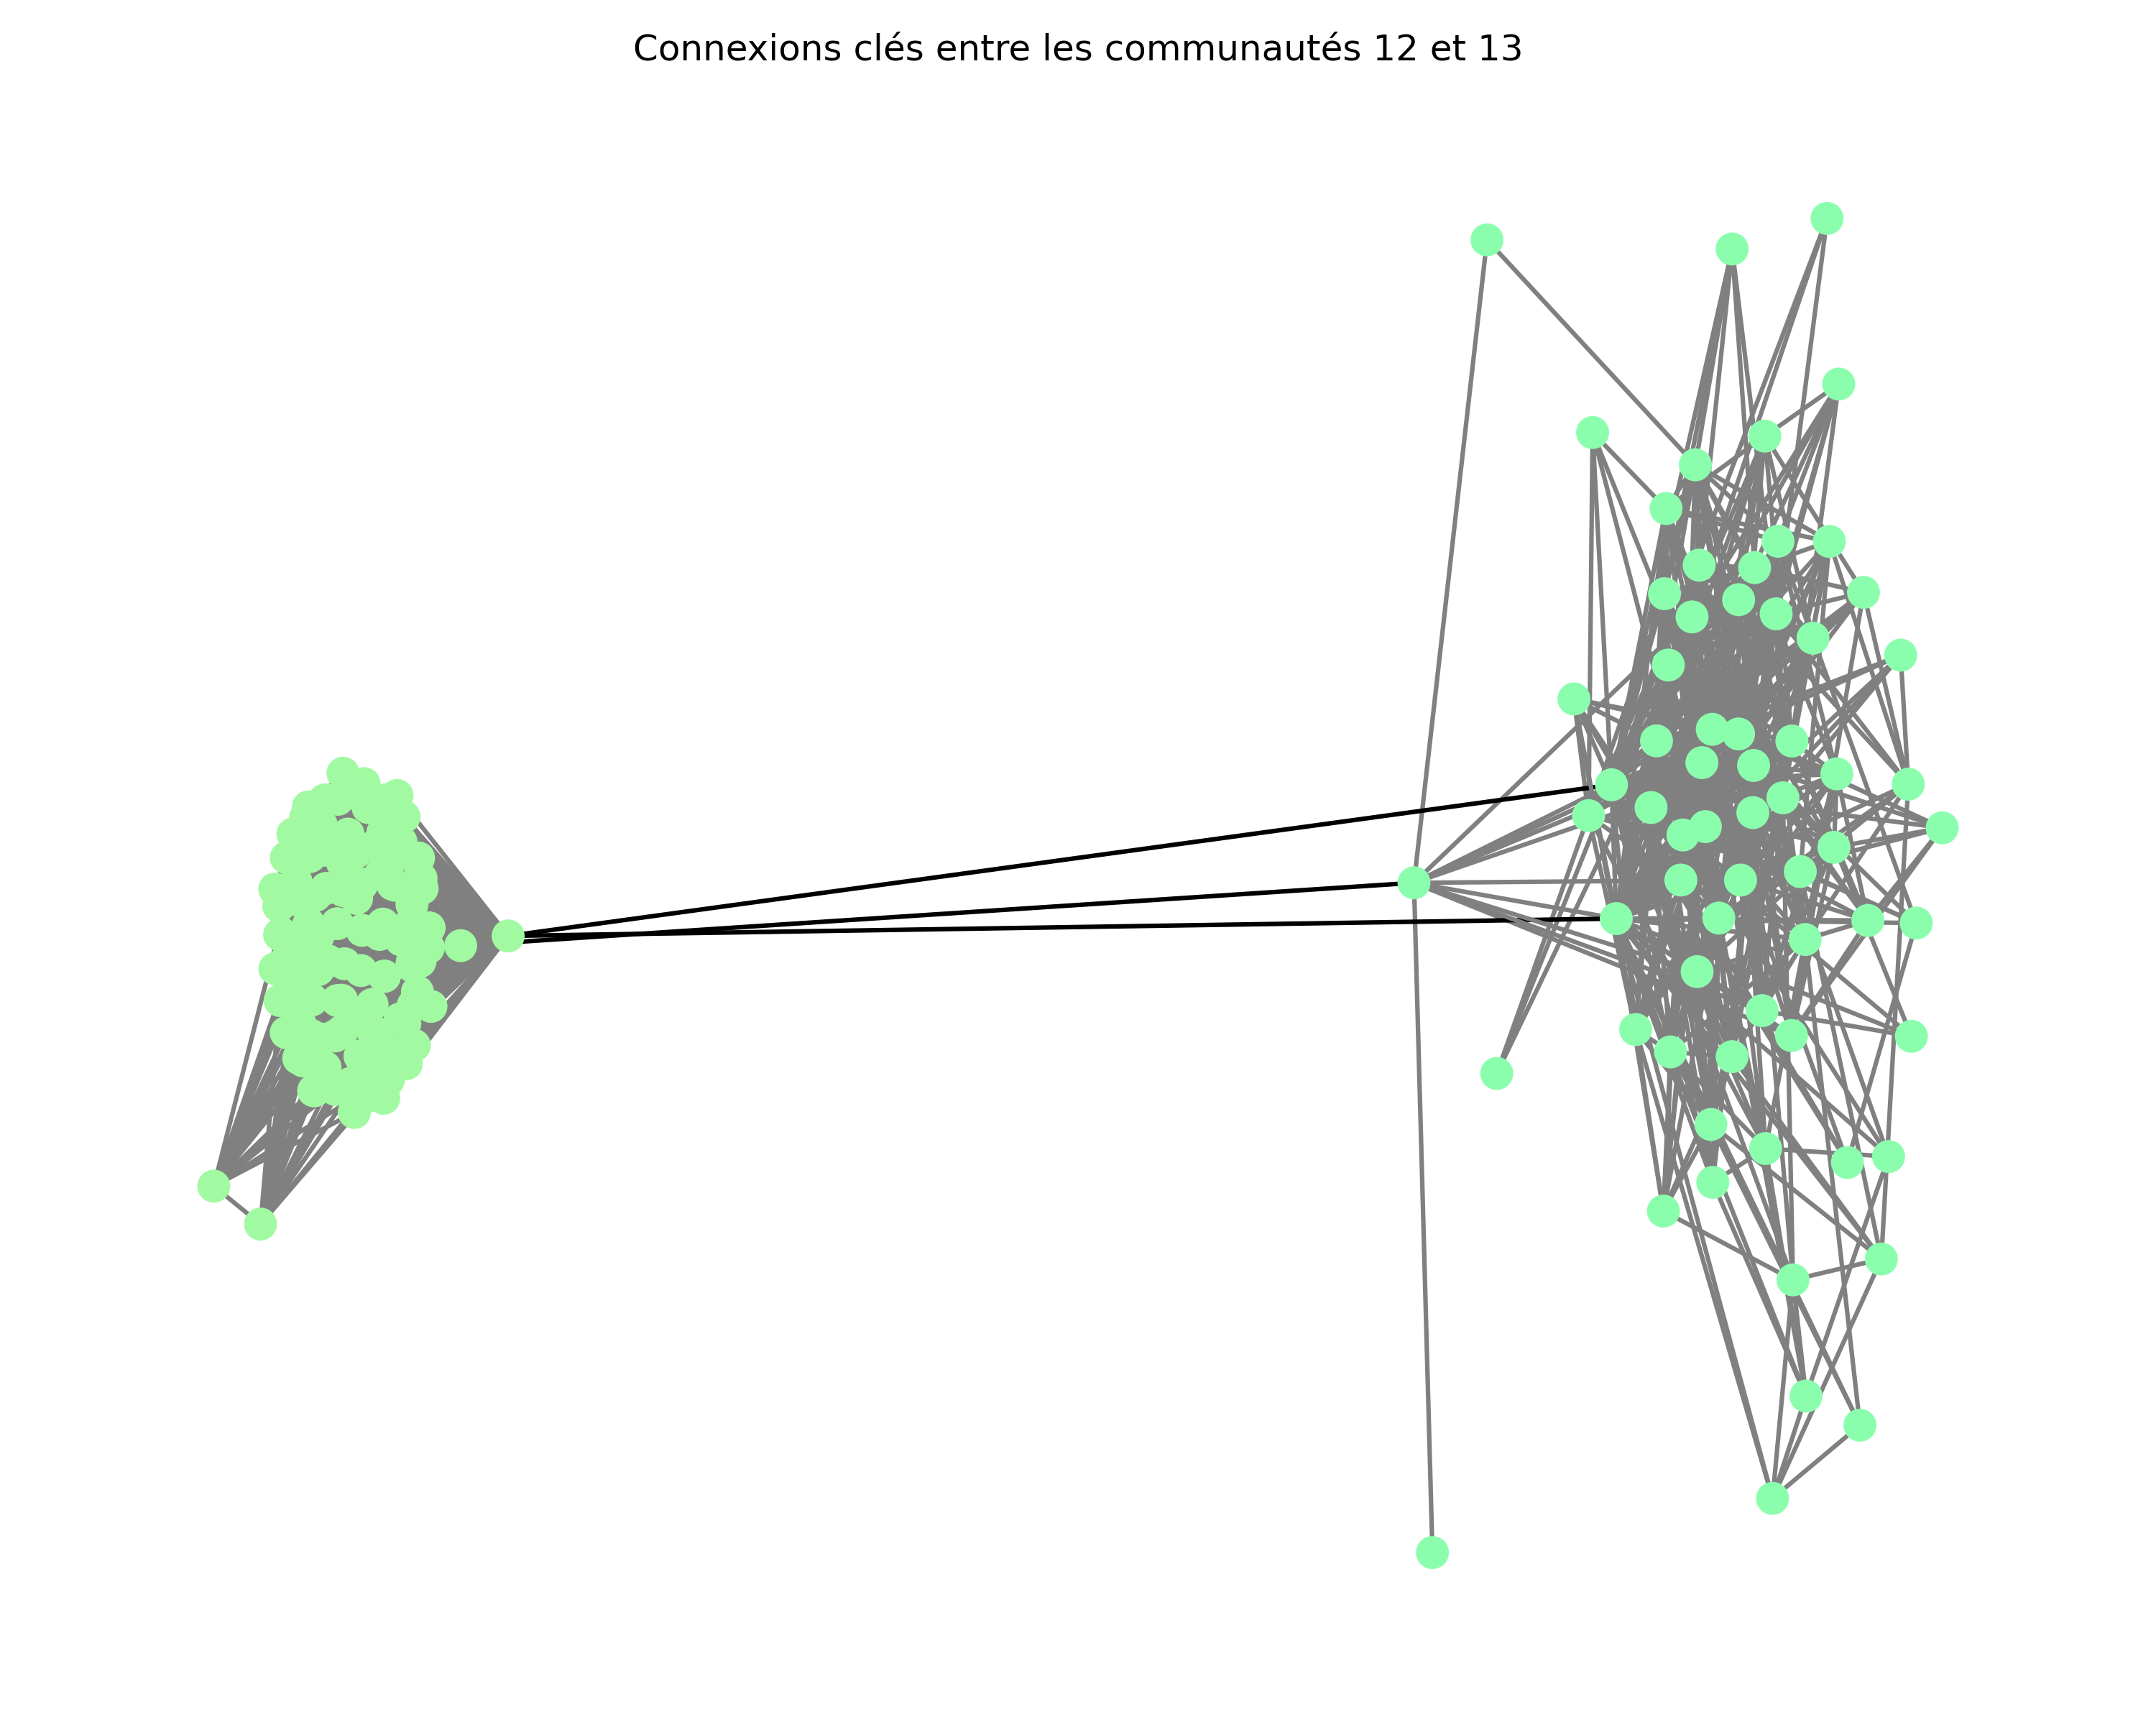
\includegraphics[width=0.8\textwidth]{liaison_12_13.png}
    \caption{Connexions clés entre les communautés 12 et 13}
    \label{fig:liaison_12_13}
\end{figure}

\vspace{1em}
Chaque image représente un sous-graphe où :
\begin{itemize}
    \item Les nœuds sont colorés selon leur communauté d’origine.
    \item Les \textbf{arêtes noires} correspondent aux connexions directes entre deux communautés.
    \item Les \textbf{arêtes grises} représentent les connexions locales (intra-communautaires) servant de contexte.
\end{itemize}

\vspace{1em}
\noindent
\textbf{Interprétation.} Ces visualisations permettent d’identifier les nœuds stratégiques jouant un rôle de \textit{connecteurs inter-groupes}. Ces derniers constituent souvent des relais d’information importants dans un contexte social, professionnel ou informationnel. L’étude de ces ponts peut s’avérer précieuse pour notre problématique.








\subsection{Identification des rôles et visualisation d'un sous-graphe optimisé}

Dans cette section, nous allons explorer les rôles des nœuds dans le réseau à l'aide de deux métriques clés : le \textbf{degré} et la \textbf{centralité d'intermédiation} (\textit{betweenness}). Ces indicateurs permettent de classer les nœuds en trois catégories :

\begin{itemize}
    \item \textbf{Leader local} : nœuds très connectés au sein de leur communauté.
    \item \textbf{Ambassadeur} : nœuds jouant un rôle de pont entre communautés.
    \item \textbf{Satellite} : nœuds périphériques avec moins de connexions.
\end{itemize}

L’objectif est de générer un \textbf{sous-graphe optimisé} mettant en lumière les connexions stratégiques entre ces différents rôles.

\subsubsection*{Étapes de l’analyse}

\begin{enumerate}
    \item Création d’un DataFrame contenant pour chaque nœud : son degré, sa centralité d’intermédiation et sa communauté.
    \item Normalisation des métriques avec \texttt{MinMaxScaler}.
    \item Attribution d’un rôle à chaque nœud selon des seuils prédéfinis.
    \item Sélection des \textit{Leaders} et \textit{Ambassadeurs}, et ajout de leurs \textit{Satellites} les plus connectés.
    \item Visualisation du sous-graphe ainsi construit.
\end{enumerate}

\subsubsection*{Code Python}

\begin{lstlisting}[language=Python, basicstyle=\small\ttfamily]
from sklearn.preprocessing import MinMaxScaler

# Création du DataFrame des nœuds
df_nodes = pd.DataFrame({
    "Node": list(G.nodes),
    "Degree": [degree[n] for n in G.nodes],
    "Betweenness": [betweenness[n] for n in G.nodes],
    "Community": [partition[n] for n in G.nodes]
})

# Normalisation
scaler = MinMaxScaler()
df_nodes[["NormDegree", "NormBetweenness"]] = scaler.fit_transform(
    df_nodes[["Degree", "Betweenness"]]
)

# Attribution des rôles
def get_role(row):
    if row["NormBetweenness"] > 0.6:
        return "Ambassadeur"
    elif row["NormDegree"] > 0.75:
        return "Leader local"
    else:
        return "Satellite"

df_nodes["Role"] = df_nodes.apply(get_role, axis=1)

# Sélection des nœuds clés et satellites les plus connectés
key_nodes = df_nodes[df_nodes["Role"].isin(["Leader local", "Ambassadeur"])]["Node"]
selected_nodes = set(key_nodes)

for node in key_nodes:
    neighbors = list(G.neighbors(node))
    satellites = [n for n in neighbors if df_nodes.loc[df_nodes["Node"] == n, "Role"].values[0] == "Satellite"]
    top_satellites = sorted(satellites, key=lambda x: degree[x], reverse=True)[:20]
    selected_nodes.update(top_satellites)

# Sous-graphe final
subG = G.subgraph(selected_nodes)
df_sub = df_nodes[df_nodes["Node"].isin(subG.nodes)].copy()

# Visualisation
pos = nx.spring_layout(subG, seed=42)
color_map = {
    "Leader local": "#e74c3c",
    "Ambassadeur": "#2980b9",
    "Satellite": "#95a5a6"
}
colors = df_sub["Role"].map(color_map)
sizes = 200 + df_sub["NormDegree"] * 10

labels = {
    row["Node"]: row["Role"]
    for _, row in df_sub.iterrows()
    if row["Role"] != "Satellite"
}

plt.figure(figsize=(16, 12))
nx.draw_networkx_nodes(subG, pos, node_color=colors, node_size=sizes, alpha=0.9)
nx.draw_networkx_edges(subG, pos, alpha=0.25, width=0.7)

# Légende
from matplotlib.patches import Patch
legend_elements = [
    Patch(color=color_map["Leader local"], label="Leader local"),
    Patch(color=color_map["Ambassadeur"], label="Ambassadeur"),
    Patch(color=color_map["Satellite"], label="Satellite")
]
plt.legend(handles=legend_elements, loc="upper right", fontsize=12)

plt.title("Leadership et satellites filtrés", fontsize=16)
plt.axis("off")
plt.tight_layout()
plt.savefig("smart_roles_graph_reduced_satellites.png", dpi=300)
plt.show()
\end{lstlisting}

\subsubsection*{Résultat visuel}

\begin{figure}[H]
    \centering
    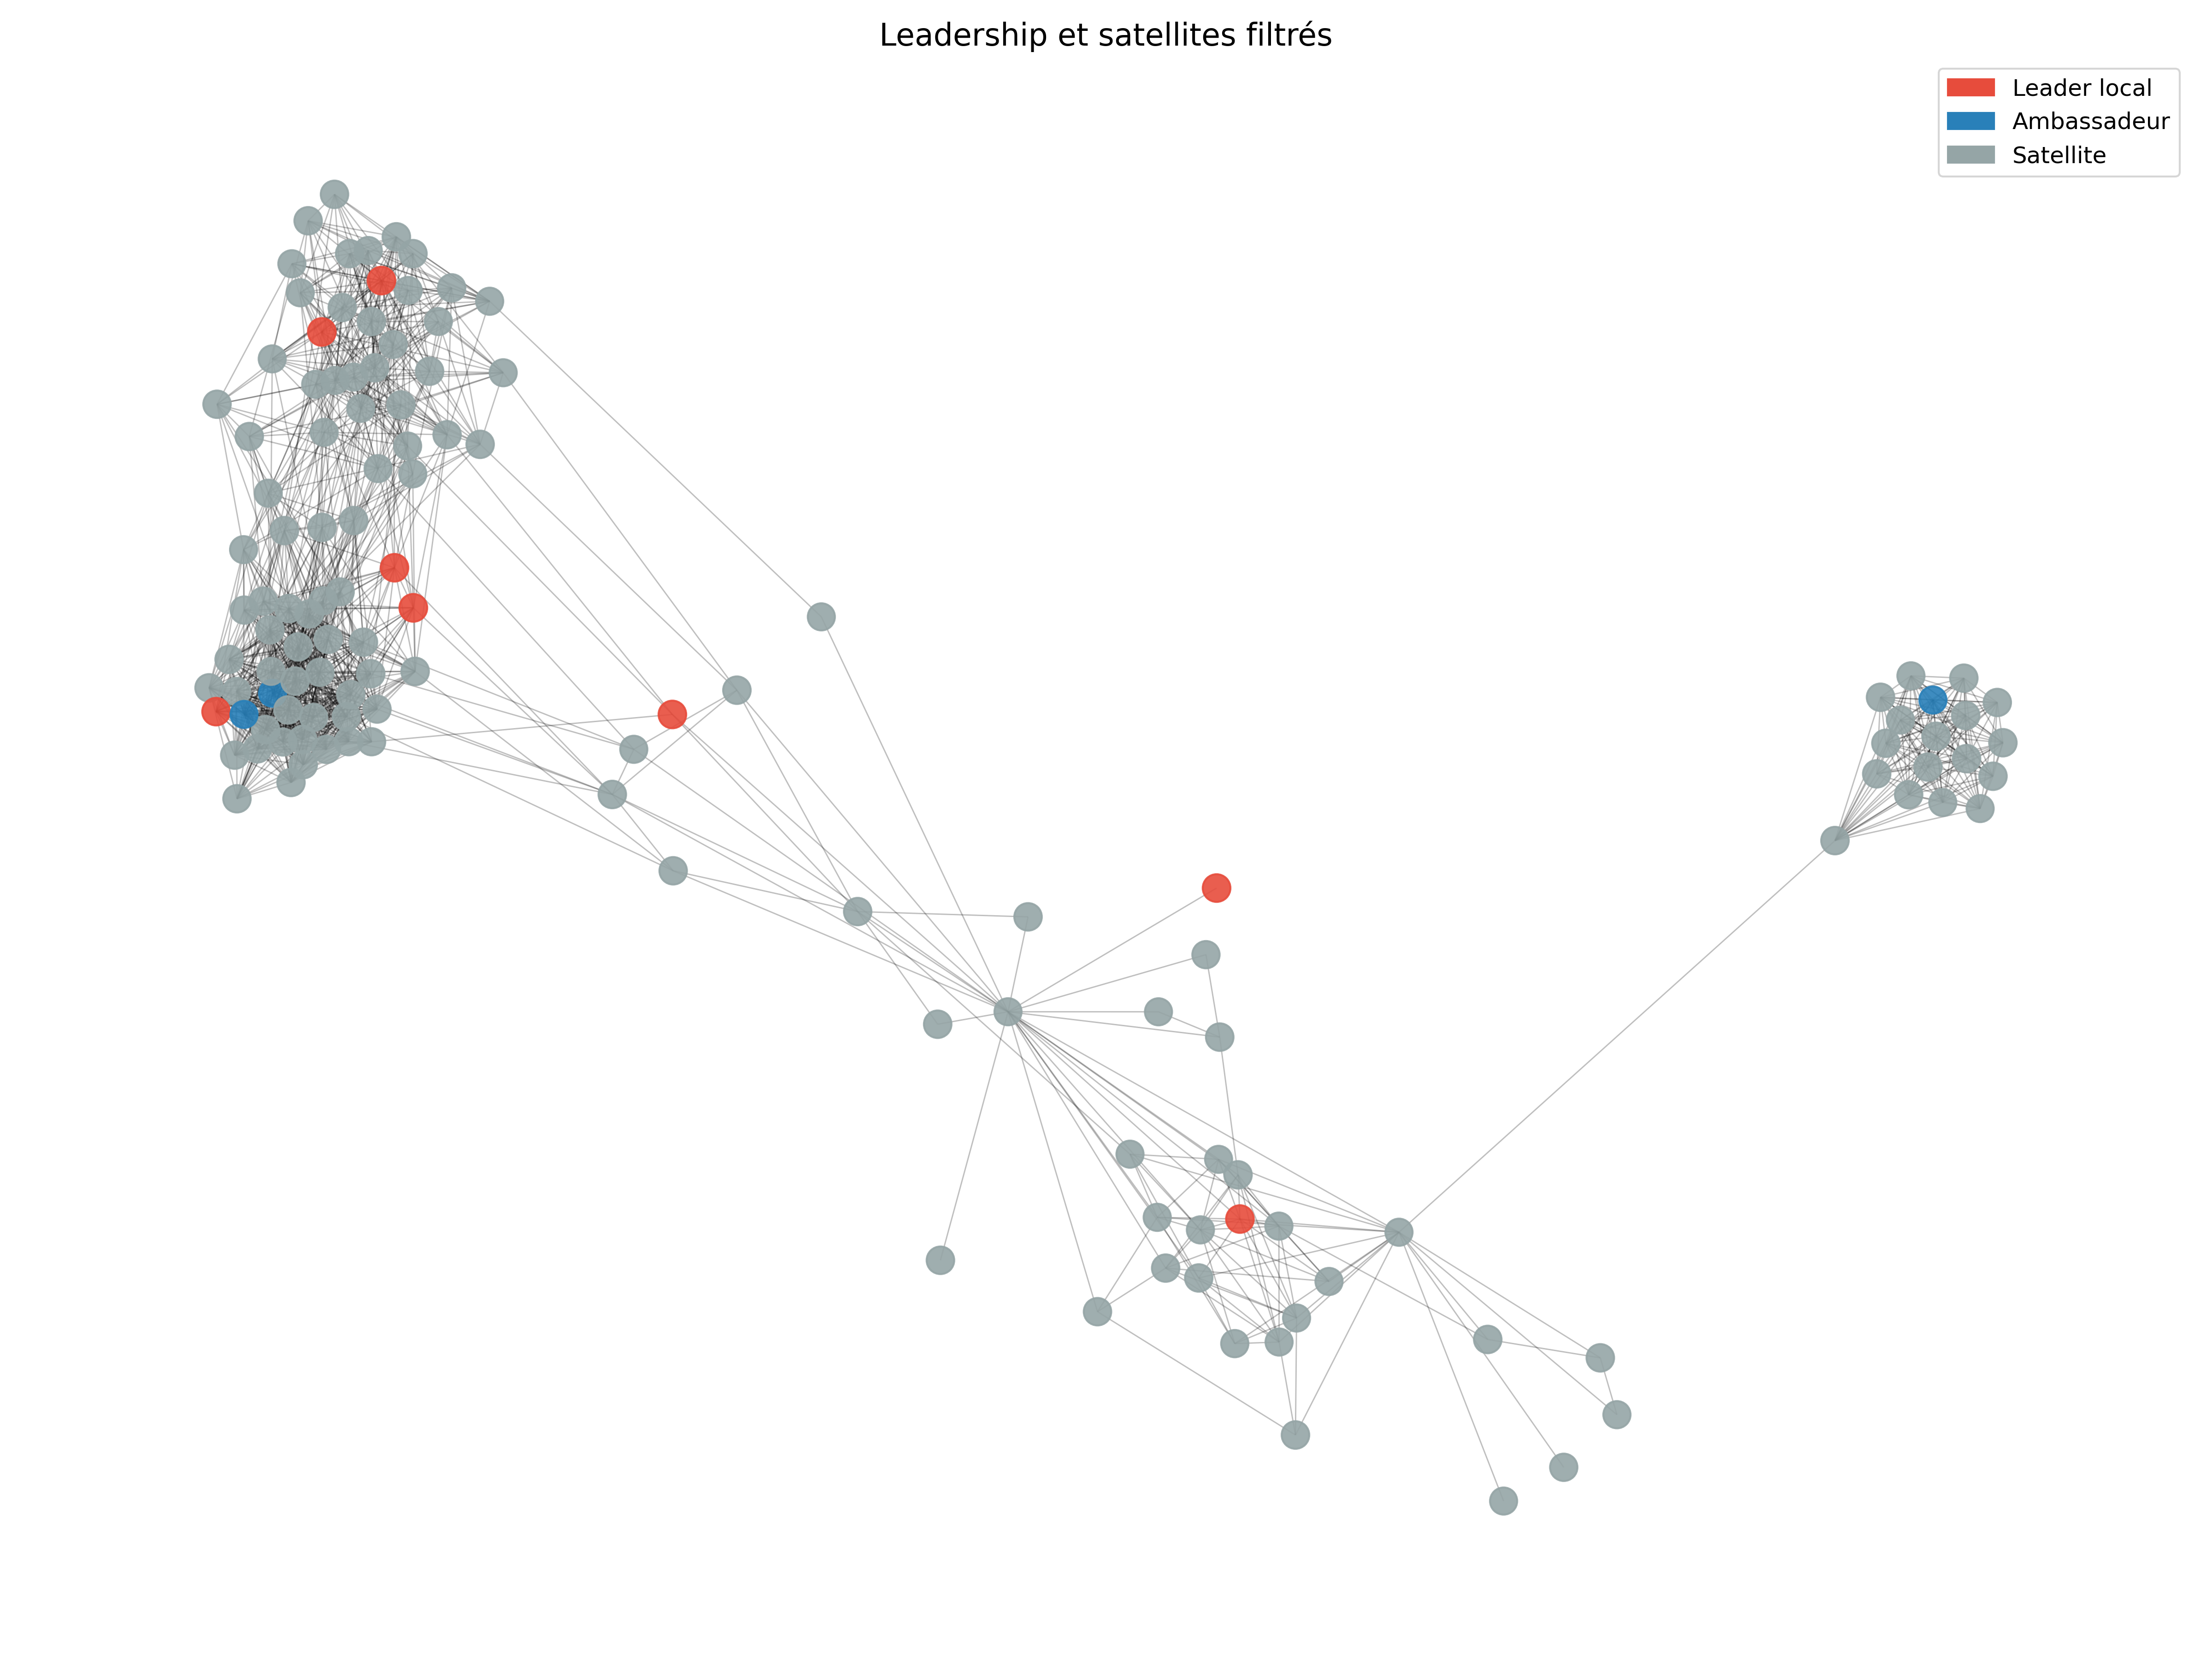
\includegraphics[width=0.8\textwidth]{smart_roles_graph_reduced_satellites.png}
    \caption{Visualisation des rôles dans le réseau : Leaders locaux, Ambassadeurs et Satellites}
    \label{fig:smart_roles}
\end{figure}

\subsubsection*{Interprétation}

\begin{itemize}
    \item \textcolor{red}{\textbf{Leaders locaux}} : au centre des interactions dans leur communauté, ils assurent une forte cohésion interne.
    \item \textcolor{blue}{\textbf{Ambassadeurs}} : véritables ponts entre communautés, ils favorisent la circulation de l’information dans le réseau.
    \item \textcolor{gray}{\textbf{Satellites}} : moins connectés, ils restent néanmoins pertinents en tant que soutiens locaux.
\end{itemize}

Cette représentation offre une lecture stratégique de la structure du réseau. En distinguant les rôles, elle met en évidence les points de pouvoir et les passerelles essentielles à l’interconnexion des communautés.


\section{Difficultés rencontrées}
Au fil du projet, nous avons été confrontés à plusieurs types de difficultés, aussi bien liées aux données qu’aux outils ou aux ressources matérielles. 

\subsection{difficultés de traitement des données}
Les données brutes que nous avons utilisées étaient massives (plus de 50 millions de lignes) et au format .txt, ce qui les rendait peu exploitables dans leur état initial. Nous avons donc dû commencer par les nettoyer et les transformer. Cela a impliqué de convertir le fichier en .csv, de supprimer les boucles, de filtrer les doublons, et surtout de conserver uniquement les relations réciproques, c’est-à-dire celles où deux utilisateurs sont amis dans les deux sens.

\subsection{Difficultés matérielles}

\subsubsection{génération du graphe}
L’un des principaux défis a été la construction du graphe complet, qui demandait beaucoup de mémoire. Sur un ordinateur personnel, il était tout simplement impossible de charger les 4 millions de nœuds et 50 millions de relations dans leur totalité. Nous avons donc dû adapter notre méthode en extrayant des sous-graphes représentatifs à partir de différentes stratégies d’échantillonnage. Cela nous a permis de travailler sur des volumes plus raisonnables tout en conservant la structure du réseau global.

\subsubsection{contrainte logicielle}
Nous avons remarqué que NetworkX, bien qu’intuitif et pratique pour des graphes de taille moyenne, ne supporte pas bien les très gros volumes. Les calculs devenaient très lents, voire impossibles à exécuter sans planter.
Pour contourner cette limite, nous avons tenté d’utiliser Neo4j, qui est beaucoup mieux adapté à la gestion de grands graphes. Cela dit, même si Neo4j s’est révélé très prometteur, nous n’avons pas pu en exploiter son potentiel. Nous avons alors continué sur NetworkX.

 
\section{Bilan}
	\subsection{Conclusion}
    Les résultats de nos analyses montrent que, bien que tous les utilisateurs très connectés ne soient pas nécessairement des ponts entre communautés, une proportion significative d’entre eux occupe cette fonction stratégique. Grâce à la combinaison des mesures de centralité, des liens inter-communautés et de la visualisation du réseau, nous avons pu mettre en évidence plusieurs "ambassadeurs" qui assurent la liaison entre des groupes qui, autrement, seraient peu ou pas connectés.\\

Ces individus jouent un rôle fondamental dans la diffusion de l’information, la structuration du réseau et le maintien de la cohésion globale. Ils constituent des cibles potentielles pour des actions comme la communication virale, l’analyse d’influence ou la prévention de fragmentation du réseau.
Nous pouvons donc conclure que, oui, les personnes ayant beaucoup d’amis ont souvent un rôle de connecteurs entre différentes communautés, même si ce rôle dépend également de la position topologique du nœud dans le graphe et non uniquement de son degré.
	\subsection{Perspectives}
    Pour aller plus loin nous pourrions étudier l’évolution temporelle du graphe, afin de voir comment les rôles de connecteurs évoluent dans le temps : certains utilisateurs deviennent-ils des ponts à mesure qu’ils se connectent à de nouveaux groupes ? Inversement, d’autres perdent-ils cette position stratégique ? 
	


\newpage
% \section{Bibliographie}
% \renewcommand{\bibname}{}
% \renewcommand{\refname}{}
% \begin{thebibliography}{2}
%    \bibitem[label]{cle} Auteur, TITRE, editeur, annee
%    \bibitem[LAM94]{lam1} L. LAMPORT, {\it \LaTeX : A Document preparation system, Addison-Wesley, 1994}
% \end{thebibliography}

% \newpage
% \section{Webographie}
% \begin{thebibliography}{2}
%    \bibitem[CAT]{cat} \url{savoircoder.fr/cat}
% \end{thebibliography}


% \newpage
% \section{Annexes}
% \appendix
% \makeatletter
% \def\@seccntformat#1{Annexe~\csname the#1\endcsname:\quad}
% \makeatother
% 	\section{Cahier des charges}
% 	\section{Exemple d'exécution du projet}
% 	\section{Manuel utilisateur}


\end{document}